\documentclass[conference]{IEEEtran}
\IEEEoverridecommandlockouts
% The preceding line is only needed to identify funding in the first footnote. If that is unneeded, please comment it out.
%Template version as of 6/27/2024

% basic
%\usepackage{color,xcolor}
\usepackage{color}
\usepackage{epsfig}
\usepackage{graphicx}
\usepackage{algorithm,algorithmic}
% \usepackage{algpseudocode}
%\usepackage{ulem}

% figure and table
\usepackage{adjustbox}
\usepackage{array}
\usepackage{booktabs}
\usepackage{colortbl}
\usepackage{float,wrapfig}
\usepackage{framed}
\usepackage{hhline}
\usepackage{multirow}
% \usepackage{subcaption} % issues a warning with CVPR/ICCV format
% \usepackage[font=small]{caption}
\usepackage[percent]{overpic}
%\usepackage{tikz} % conflict with ECCV format

% font and character
\usepackage{amsmath,amsfonts,amssymb}
% \let\proof\relax      % for ECCV llncs class
% \let\endproof\relax   % for ECCV llncs class
\usepackage{amsthm} 
\usepackage{bm}
\usepackage{nicefrac}
\usepackage{microtype}
\usepackage{contour}
\usepackage{courier}
%\usepackage{palatino}
%\usepackage{times}

% layout
\usepackage{changepage}
\usepackage{extramarks}
\usepackage{fancyhdr}
\usepackage{lastpage}
\usepackage{setspace}
\usepackage{soul}
\usepackage{xspace}
\usepackage{cuted}
\usepackage{fancybox}
\usepackage{afterpage}
%\usepackage{enumitem} % conflict with IEEE format
%\usepackage{titlesec} % conflict with ECCV format

% ref
% commenting these two out for this submission so it looks the same as RSS example
% \usepackage[breaklinks=true,colorlinks,backref=True]{hyperref}
% \hypersetup{colorlinks,linkcolor={black},citecolor={MSBlue},urlcolor={magenta}}
\usepackage{url}
\usepackage{quoting}
\usepackage{epigraph}

% misc
\usepackage{enumerate}
\usepackage{paralist,tabularx}
\usepackage{comment}
\usepackage{pdfpages}
% \usepackage[draft]{todonotes} % conflict with CVPR/ICCV/ECCV format



% \usepackage{todonotes}
% \usepackage{caption}
% \usepackage{subcaption}

\usepackage{pifont}% http://ctan.org/pkg/pifont

% extra symbols
\usepackage{MnSymbol}



\def\BibTeX{{\rm B\kern-.05em{\sc i\kern-.025em b}\kern-.08em
    T\kern-.1667em\lower.7ex\hbox{E}\kern-.125emX}}
\begin{document}

\title{Implicit Communication in Human-Robot Collaborative Transport}

\author{
\IEEEauthorblockN{Elvin Yang}
\IEEEauthorblockA{
    \textit{Department of Robotics} \\
    \textit{University of Michigan} \\
    Ann Arbor, MI, USA \\
    eyy@umich.edu
}
\and
\IEEEauthorblockN{Christoforos Mavrogiannis}
\IEEEauthorblockA{
    \textit{Department of Robotics} \\
    \textit{University of Michigan} \\
    Ann Arbor, MI, USA \\
    cmavro@umich.edu
}
}

\maketitle

\begin{abstract}  
Test time scaling is currently one of the most active research areas that shows promise after training time scaling has reached its limits.
Deep-thinking (DT) models are a class of recurrent models that can perform easy-to-hard generalization by assigning more compute to harder test samples.
However, due to their inability to determine the complexity of a test sample, DT models have to use a large amount of computation for both easy and hard test samples.
Excessive test time computation is wasteful and can cause the ``overthinking'' problem where more test time computation leads to worse results.
In this paper, we introduce a test time training method for determining the optimal amount of computation needed for each sample during test time.
We also propose Conv-LiGRU, a novel recurrent architecture for efficient and robust visual reasoning. 
Extensive experiments demonstrate that Conv-LiGRU is more stable than DT, effectively mitigates the ``overthinking'' phenomenon, and achieves superior accuracy.
\end{abstract}  

% HRI2025 requests that we use semicolons as delimiters instead of commas.
\begin{IEEEkeywords}
Human-robot collaboration; Human-robot teams; Implicit communication
\end{IEEEkeywords}

\section{Introduction}
\label{sec:introduction}
The business processes of organizations are experiencing ever-increasing complexity due to the large amount of data, high number of users, and high-tech devices involved \cite{martin2021pmopportunitieschallenges, beerepoot2023biggestbpmproblems}. This complexity may cause business processes to deviate from normal control flow due to unforeseen and disruptive anomalies \cite{adams2023proceddsriftdetection}. These control-flow anomalies manifest as unknown, skipped, and wrongly-ordered activities in the traces of event logs monitored from the execution of business processes \cite{ko2023adsystematicreview}. For the sake of clarity, let us consider an illustrative example of such anomalies. Figure \ref{FP_ANOMALIES} shows a so-called event log footprint, which captures the control flow relations of four activities of a hypothetical event log. In particular, this footprint captures the control-flow relations between activities \texttt{a}, \texttt{b}, \texttt{c} and \texttt{d}. These are the causal ($\rightarrow$) relation, concurrent ($\parallel$) relation, and other ($\#$) relations such as exclusivity or non-local dependency \cite{aalst2022pmhandbook}. In addition, on the right are six traces, of which five exhibit skipped, wrongly-ordered and unknown control-flow anomalies. For example, $\langle$\texttt{a b d}$\rangle$ has a skipped activity, which is \texttt{c}. Because of this skipped activity, the control-flow relation \texttt{b}$\,\#\,$\texttt{d} is violated, since \texttt{d} directly follows \texttt{b} in the anomalous trace.
\begin{figure}[!t]
\centering
\includegraphics[width=0.9\columnwidth]{images/FP_ANOMALIES.png}
\caption{An example event log footprint with six traces, of which five exhibit control-flow anomalies.}
\label{FP_ANOMALIES}
\end{figure}

\subsection{Control-flow anomaly detection}
Control-flow anomaly detection techniques aim to characterize the normal control flow from event logs and verify whether these deviations occur in new event logs \cite{ko2023adsystematicreview}. To develop control-flow anomaly detection techniques, \revision{process mining} has seen widespread adoption owing to process discovery and \revision{conformance checking}. On the one hand, process discovery is a set of algorithms that encode control-flow relations as a set of model elements and constraints according to a given modeling formalism \cite{aalst2022pmhandbook}; hereafter, we refer to the Petri net, a widespread modeling formalism. On the other hand, \revision{conformance checking} is an explainable set of algorithms that allows linking any deviations with the reference Petri net and providing the fitness measure, namely a measure of how much the Petri net fits the new event log \cite{aalst2022pmhandbook}. Many control-flow anomaly detection techniques based on \revision{conformance checking} (hereafter, \revision{conformance checking}-based techniques) use the fitness measure to determine whether an event log is anomalous \cite{bezerra2009pmad, bezerra2013adlogspais, myers2018icsadpm, pecchia2020applicationfailuresanalysispm}. 

The scientific literature also includes many \revision{conformance checking}-independent techniques for control-flow anomaly detection that combine specific types of trace encodings with machine/deep learning \cite{ko2023adsystematicreview, tavares2023pmtraceencoding}. Whereas these techniques are very effective, their explainability is challenging due to both the type of trace encoding employed and the machine/deep learning model used \cite{rawal2022trustworthyaiadvances,li2023explainablead}. Hence, in the following, we focus on the shortcomings of \revision{conformance checking}-based techniques to investigate whether it is possible to support the development of competitive control-flow anomaly detection techniques while maintaining the explainable nature of \revision{conformance checking}.
\begin{figure}[!t]
\centering
\includegraphics[width=\columnwidth]{images/HIGH_LEVEL_VIEW.png}
\caption{A high-level view of the proposed framework for combining \revision{process mining}-based feature extraction with dimensionality reduction for control-flow anomaly detection.}
\label{HIGH_LEVEL_VIEW}
\end{figure}

\subsection{Shortcomings of \revision{conformance checking}-based techniques}
Unfortunately, the detection effectiveness of \revision{conformance checking}-based techniques is affected by noisy data and low-quality Petri nets, which may be due to human errors in the modeling process or representational bias of process discovery algorithms \cite{bezerra2013adlogspais, pecchia2020applicationfailuresanalysispm, aalst2016pm}. Specifically, on the one hand, noisy data may introduce infrequent and deceptive control-flow relations that may result in inconsistent fitness measures, whereas, on the other hand, checking event logs against a low-quality Petri net could lead to an unreliable distribution of fitness measures. Nonetheless, such Petri nets can still be used as references to obtain insightful information for \revision{process mining}-based feature extraction, supporting the development of competitive and explainable \revision{conformance checking}-based techniques for control-flow anomaly detection despite the problems above. For example, a few works outline that token-based \revision{conformance checking} can be used for \revision{process mining}-based feature extraction to build tabular data and develop effective \revision{conformance checking}-based techniques for control-flow anomaly detection \cite{singh2022lapmsh, debenedictis2023dtadiiot}. However, to the best of our knowledge, the scientific literature lacks a structured proposal for \revision{process mining}-based feature extraction using the state-of-the-art \revision{conformance checking} variant, namely alignment-based \revision{conformance checking}.

\subsection{Contributions}
We propose a novel \revision{process mining}-based feature extraction approach with alignment-based \revision{conformance checking}. This variant aligns the deviating control flow with a reference Petri net; the resulting alignment can be inspected to extract additional statistics such as the number of times a given activity caused mismatches \cite{aalst2022pmhandbook}. We integrate this approach into a flexible and explainable framework for developing techniques for control-flow anomaly detection. The framework combines \revision{process mining}-based feature extraction and dimensionality reduction to handle high-dimensional feature sets, achieve detection effectiveness, and support explainability. Notably, in addition to our proposed \revision{process mining}-based feature extraction approach, the framework allows employing other approaches, enabling a fair comparison of multiple \revision{conformance checking}-based and \revision{conformance checking}-independent techniques for control-flow anomaly detection. Figure \ref{HIGH_LEVEL_VIEW} shows a high-level view of the framework. Business processes are monitored, and event logs obtained from the database of information systems. Subsequently, \revision{process mining}-based feature extraction is applied to these event logs and tabular data input to dimensionality reduction to identify control-flow anomalies. We apply several \revision{conformance checking}-based and \revision{conformance checking}-independent framework techniques to publicly available datasets, simulated data of a case study from railways, and real-world data of a case study from healthcare. We show that the framework techniques implementing our approach outperform the baseline \revision{conformance checking}-based techniques while maintaining the explainable nature of \revision{conformance checking}.

In summary, the contributions of this paper are as follows.
\begin{itemize}
    \item{
        A novel \revision{process mining}-based feature extraction approach to support the development of competitive and explainable \revision{conformance checking}-based techniques for control-flow anomaly detection.
    }
    \item{
        A flexible and explainable framework for developing techniques for control-flow anomaly detection using \revision{process mining}-based feature extraction and dimensionality reduction.
    }
    \item{
        Application to synthetic and real-world datasets of several \revision{conformance checking}-based and \revision{conformance checking}-independent framework techniques, evaluating their detection effectiveness and explainability.
    }
\end{itemize}

The rest of the paper is organized as follows.
\begin{itemize}
    \item Section \ref{sec:related_work} reviews the existing techniques for control-flow anomaly detection, categorizing them into \revision{conformance checking}-based and \revision{conformance checking}-independent techniques.
    \item Section \ref{sec:abccfe} provides the preliminaries of \revision{process mining} to establish the notation used throughout the paper, and delves into the details of the proposed \revision{process mining}-based feature extraction approach with alignment-based \revision{conformance checking}.
    \item Section \ref{sec:framework} describes the framework for developing \revision{conformance checking}-based and \revision{conformance checking}-independent techniques for control-flow anomaly detection that combine \revision{process mining}-based feature extraction and dimensionality reduction.
    \item Section \ref{sec:evaluation} presents the experiments conducted with multiple framework and baseline techniques using data from publicly available datasets and case studies.
    \item Section \ref{sec:conclusions} draws the conclusions and presents future work.
\end{itemize}

%\section{Related Work}
%\label{sec:related-work}

%\subsection{Background}

%Defect detection is critical to ensure the yield of integrated circuit manufacturing lines and reduce faults. Previous research has primarily focused on wafer map data, which engineers produce by marking faulty chips with different colors based on test results. The specific spatial distribution of defects on a wafer can provide insights into the causes, thereby helping to determine which stage of the manufacturing process is responsible for the issues. Although such research is relatively mature, the continual miniaturization of integrated circuits and the increasing complexity and density of chip components have made chip-level detection more challenging, leading to potential risks\cite{ma2023review}. Consequently, there is a need to combine this approach with magnified imaging of the wafer surface using scanning electron microscopes (SEMs) to detect, classify, and analyze specific microscopic defects, thus helping to identify the particular process steps where defects originate.

%Previously, wafer surface defect classification and detection were primarily conducted by experienced engineers. However, this method relies heavily on the engineers' expertise and involves significant time expenditure and subjectivity, lacking uniform standards. With the ongoing development of artificial intelligence, deep learning methods using multi-layer neural networks to extract and learn target features have proven highly effective for this task\cite{gao2022review}.

%In the task of defect classification, it is typical to use a model structure that initially extracts features through convolutional and pooling layers, followed by classification via fully connected layers. Researchers have recently developed numerous classification model structures tailored to specific problems. These models primarily focus on how to extract defect features effectively. For instance, Chen et al. presented a defect recognition and classification algorithm rooted in PCA and classification SVM\cite{chen2008defect}. Chang et al. utilized SVM, drawing on features like smoothness and texture intricacy, for classifying high-intensity defect images\cite{chang2013hybrid}. The classification of defect images requires the formulation of numerous classifiers tailored for myriad inspection steps and an Abundance of accurately labeled data, making data acquisition challenging. Cheon et al. proposed a single CNN model adept at feature extraction\cite{cheon2019convolutional}. They achieved a granular classification of wafer surface defects by recognizing misclassified images and employing a k-nearest neighbors (k-NN) classifier algorithm to gauge the aggregate squared distance between each image feature vector and its k-neighbors within the same category. However, when applied to new or unseen defects, such models necessitate retraining, incurring computational overheads. Moreover, with escalating CNN complexity, the computational demands surge.

%Segmentation of defects is necessary to locate defect positions and gather information such as the size of defects. Unlike classification networks, segmentation networks often use classic encoder-decoder structures such as UNet\cite{ronneberger2015u} and SegNet\cite{badrinarayanan2017segnet}, which focus on effectively leveraging both local and global feature information. Han Hui et al. proposed integrating a Region Proposal Network (RPN) with a UNet architecture to suggest defect areas before conducting defect segmentation \cite{han2020polycrystalline}. This approach enables the segmentation of various defects in wafers with only a limited set of roughly labeled images, enhancing the efficiency of training and application in environments where detailed annotations are scarce. Subhrajit Nag et al. introduced a new network structure, WaferSegClassNet, which extracts multi-scale local features in the encoder and performs classification and segmentation tasks in the decoder \cite{nag2022wafersegclassnet}. This model represents the first detection system capable of simultaneously classifying and segmenting surface defects on wafers. However, it relies on extensive data training and annotation for high accuracy and reliability. 

%Recently, Vic De Ridder et al. introduced a novel approach for defect segmentation using diffusion models\cite{de2023semi}. This approach treats the instance segmentation task as a denoising process from noise to a filter, utilizing diffusion models to predict and reconstruct instance masks for semiconductor defects. This method achieves high precision and improved defect classification and segmentation detection performance. However, the complex network structure and the computational process of the diffusion model require substantial computational resources. Moreover, the performance of this model heavily relies on high-quality and large amounts of training data. These issues make it less suitable for industrial applications. Additionally, the model has only been applied to detecting and segmenting a single type of defect(bridges) following a specific manufacturing process step, limiting its practical utility in diverse industrial scenarios.

%\subsection{Few-shot Anomaly Detection}
%Traditional anomaly detection techniques typically rely on extensive training data to train models for identifying and locating anomalies. However, these methods often face limitations in rapidly changing production environments and diverse anomaly types. Recent research has started exploring effective anomaly detection using few or zero samples to address these challenges.

%Huang et al. developed the anomaly detection method RegAD, based on image registration technology. This method pre-trains an object-agnostic registration network with various images to establish the normality of unseen objects. It identifies anomalies by aligning image features and has achieved promising results. Despite these advancements, implementing few-shot settings in anomaly detection remains an area ripe for further exploration. Recent studies show that pre-trained vision-language models such as CLIP and MiniGPT can significantly enhance performance in anomaly detection tasks.

%Dong et al. introduced the MaskCLIP framework, which employs masked self-distillation to enhance contrastive language-image pretraining\cite{zhou2022maskclip}. This approach strengthens the visual encoder's learning of local image patches and uses indirect language supervision to enhance semantic understanding. It significantly improves transferability and pretraining outcomes across various visual tasks, although it requires substantial computational resources.
%Jeong et al. crafted the WinCLIP framework by integrating state words and prompt templates to characterize normal and anomalous states more accurately\cite{Jeong_2023_CVPR}. This framework introduces a novel window-based technique for extracting and aggregating multi-scale spatial features, significantly boosting the anomaly detection performance of the pre-trained CLIP model.
%Subsequently, Li et al. have further contributed to the field by creating a new expansive multimodal model named Myriad\cite{li2023myriad}. This model, which incorporates a pre-trained Industrial Anomaly Detection (IAD) model to act as a vision expert, embeds anomaly images as tokens interpretable by the language model, thus providing both detailed descriptions and accurate anomaly detection capabilities.
%Recently, Chen et al. introduced CLIP-AD\cite{chen2023clip}, and Li et al. proposed PromptAD\cite{li2024promptad}, both employing language-guided, tiered dual-path model structures and feature manipulation strategies. These approaches effectively address issues encountered when directly calculating anomaly maps using the CLIP model, such as reversed predictions and highlighting irrelevant areas. Specifically, CLIP-AD optimizes the utilization of multi-layer features, corrects feature misalignment, and enhances model performance through additional linear layer fine-tuning. PromptAD connects normal prompts with anomaly suffixes to form anomaly prompts, enabling contrastive learning in a single-class setting.

%These studies extend the boundaries of traditional anomaly detection techniques and demonstrate how to effectively address rapidly changing and sample-scarce production environments through the synergy of few-shot learning and deep learning models. Building on this foundation, our research further explores wafer surface defect detection based on the CLIP model, especially focusing on achieving efficient and accurate anomaly detection in the highly specialized and variable semiconductor manufacturing process using a minimal amount of labeled data.

\section{Preliminary and MOTIVATIONS}
\label{sec:preliminary-motivations}

\subsection{Problem Statement}
\label{sec:preliminary}
We 
%first describe the dataset used in this study, and then formally 
proceed to define the Hybrid Vector Query (\hvq).

\noindent\textbf{Dataset.} We consider a dataset $D$ consisting of $N$ objects. Each object $o\in D$ is characterized by two features: (1) {\cheng one} feature vector, denoted by $o.e$,  defined in a $d$-dimensional Euclidean space $E^{d}$, where $d$ is typically hundreds, and (2) {\cheng the other} feature vector, denoted {\cheng by} $o.s$, defined in an $m$-dimensional Euclidean space $E^{m}$, where $m$ 
%can 
may vary from two to hundreds, depending on applications.


\noindent\textbf{Hybrid Vector Query (\hvq):} Given a dataset $D$, a hybrid vector query $q=\langle e, s, \alpha, k\rangle$ consists of 
% a feature vector $q.e \in E^{d}$, a feature vector $q.s \in E^{m}$, 
{\cheng two feature vectors $q.e \in E^{d}$ and $q.s \in E^{m}$,}
a hyperparameter $q.\alpha\in [0,1]$, and the number of objects to be returned $q.k$. 
%The 
\hvq aims to retrieve $k$ objects with the {\cheng minimum} 
%hybrid 
distance $Dist(q,o)$:
\begin{equation}
\begin{aligned}
    Dist(q, o) = q.\alpha \times \delta_e(q, o) + (1-q.\alpha) \times \delta_s(q, o),
\end{aligned}
\label{eq:hybird_distance}
\end{equation}
where $\delta_e(q, o)=\frac{\delta(q.e, \ o.e)}{e_{max}}$ and $\delta_s(q, o)=\frac{\delta(q.s,\ o.s)}{s_{max}}$. Here, $\delta(x, y)$ represents the Euclidean distance between vectors $x$ and $y$, and $e_{max}$ (resp. $s_{max}$) denotes the maximum Euclidean distance between $o.e$ (resp. $o.s$) of any two objects in the dataset and is used as a normalization factor. %$\alpha \in [0, 1]$ is a user-defined parameter used to balance the importance between two feature vectors. 
Following 
%existing research
previous work~\cite{milvus2021}, we use the weighted aggregated score as the similarity metric, and $q.\alpha \in [0, 1]$ is a %user-defined 
parameter that allows to set preferences between the two vectors at query time. 

\noindent\textbf{Problem Statement.} In this study, we aim to develop a graph-based ANNS index for the \hvq problem that maintains both accuracy and efficiency under %varying 
different query $\alpha$ values.


\noindent\revision{%\annotation{R1O1, R2O1, R2O2}
\textbf{Comparison of HVQ and Hybrid Queries.} Several types of hybrid queries are related to \hvq, and we next discuss their differences. %On the one hand, 
Early studies on hybrid queries~\cite{fagin2001optimal,franzke2016indexing} typically assume that each object has multiple attributes, such as price, and aim to identify the top-k objects ranked by monotone aggregation functions, e.g., the sum of these attributes. These studies %are designed for 
focus on numeric or low-dimensional attributes (e.g., geo-location) and aim to find the exact top-k results (as to be detailed in Section~\ref{sec:related}). Due to the curse of dimensionality~\cite{curse1,curse2}, they are not suitable for the \hvq problem. 
%we study. %On the other hand, 
When one of the vectors is low-dimensional coordinates, \hvq can function as semantic-aware spatial keyword queries~\cite{qianSemanticawareTopkSpatial2018}, which differ from traditional spatial keyword queries. However, existing methods for semantic-aware spatial keyword queries~\cite{chenS2RtreePivotbasedIndexing2020,qianSemanticawareTopkSpatial2018, DBLP:conf/edbt/TheodoropoulosN24} often suffer from severe efficiency challenges (as to be detailed in Section~\ref{sec:related}).}

\subsection{Graph-based ANNS methods}
\label{sec:graph-anns}

% \pasq{You wrote the exact same paragraph in the introduction, it does not look good to me.}


% To address the ANNS problem, various methods have been proposed~[xx], such as tree-based methods~[xx], hashing-based methods~[xx], quantization-based methods~[xx], and graph-based methods~[xx]. 
According to experimental evaluations~\cite{liApproximateNearestNeighbor2020, wang2021comprehensive}, graph-based approaches have demonstrated superior performance compared to other ANNS techniques. 
%Such methods 
They build a graph $G(V, E)$ where each node $x \in V$ corresponds to an object $o \in D$. The Hierarchical Navigable Small World graph (HNSW)~\cite{malkovEfficientRobustApproximate2020}, as illustrated in Figure~\ref{fig:hnsw}, is a %representative
state-of-the-art method. 
%well-known example. 
It comprises several layers, where layer 0 contains all objects, and each upper layer $i\ge1$, randomly retains a subset of the objects from layer $i-1$. Within each layer, a vertex is connected to several approximate nearest neighbors, while across adjacent layers, two vertices are connected only if they represent the same vector data.


\begin{figure}[!t]
\begin{center}
% \vspace*{-1em}
\subcaptionbox{HNSW.\label{fig:hnsw}}{
\includegraphics[width=0.35\columnwidth]{fig/HNSW.pdf}
}
% \vspace*{-1em}
\subcaptionbox{Pruning Strategy of RNG.\label{fig:rng}}{
\includegraphics[width=0.35\columnwidth]{fig/RNG-Lune.pdf}
}
% \vspace{-0.5em}
\caption{Figure~\ref{fig:hnsw} illustrates the HNSW index. Figure~\ref{fig:rng}~illustrates the pruning strategy of the Relative Neighborhood Graph (RNG).}
\label{fig:hnsw-rng}
% \vspace*{-2em}
\end{center}
\end{figure}

At %the 
query time, the HNSW algorithm starts the search from the vertex in the top layer, as shown in Figure~\ref{fig:hnsw}. %\ziqi
{At each layer, the HNSW algorithm accesses all neighbors of the current vertex and checks whether there exists a neighbor closer to the query than the current vertex. If so, it moves to the neighbor nearest to the query. This process continues within the layer until no closer neighbor to the query can be found.
%of the current vertex closer to the query. 
It then proceeds to the next layer and repeats the same procedure, using the current vertex as the starting vertex. This process continues until reaching layer 0.} 
%In the subsequent layer, it iteratively moves to the neighbor closest to the query until no neighbor closer than the current node exists. The reached node is used as the new starting point and the algorithm proceeds to the next layer until reaching layer 0. 
At layer 0, it conducts a greedy search algorithm, a method commonly used by %most 
graph-based ANNS indexes~\cite{wang2021comprehensive,fu2019fast,liApproximateNearestNeighbor2020,DBLP:journals/pami/FuWC22,DBLP:journals/is/MalkovPLK14,DBLP:conf/cvpr/HarwoodD16}. Specifically, it maintains two sets, a candidate set $\mathcal{S}$ (a min-heap) and a result set $\mathcal{R}$ (a max-heap), where $R$ stores the approximate nearest neighbors that have currently been found for the query, and $S$ stores candidates that can potentially improve $R$. At each iteration, the object with the smallest distance in $\mathcal{S}$ is popped, and its neighbors are evaluated. If a neighbor has not been visited before and its distance from the query is smaller than the maximum distance in $\mathcal{R}$, the neighbor is added to $\mathcal{S}$ and $\mathcal{R}$. Here, new elements are inserted into $\mathcal{R}$ continuously.
%without popping. 
To avoid the high maintenance cost when $\mathcal{R}$ becomes large, which would reduce search efficiency, a hyperparameter $ef_{search}$ is used to control its size. If the size of $\mathcal{R}$ exceeds $ef_{search}$, the object with the maximum distance in $\mathcal{R}$ is removed. The candidate set $\mathcal{S}$ is unbounded in size, as empirically it does not significantly reduce efficiency. The search stops and returns the $k$ nearest objects in $\mathcal{R}$ when the minimum distance in $\mathcal{S}$ is larger than the maximum distance in $\mathcal{R}$. The hyperparameter $ef_{search}$ controls the accuracy-efficiency trade-off at query time.


% The candidate set $\mathcal{S}$ is unbounded in size, while the result set $\mathcal{R}$ has its size bounded by a hyperparameter $ef_{search}$, where $ef_{search}$ controls the accuracy-efficiency trade-off.
% %during the query phase. 
% At each iteration, the object with the smallest distance in $\mathcal{S}$ is popped, and its neighbors are evaluated. If a neighbor's distance from the query is smaller than the maximum distance in $\mathcal{R}$, the neighbor is added to $\mathcal{S}$ and $\mathcal{R}$. If $\mathcal{R}$ exceeds $ef_{search}$, the object with the maximum distance in $\mathcal{R}$ is removed. The search stops and returns the $k$ nearest objects in $\mathcal{R}$ when the minimum distance in $\mathcal{S}$ is larger than the maximum distance in $\mathcal{R}$. 


% Clearly, the graph structure plays an important role %in HNSW and similarly for other graph-based indexes
Clearly, the graph structure plays a key role in graph-based ANNS indexes, as verified in the work~\cite{wang2021comprehensive}. According to~\cite{wang2021comprehensive}, 
%most 
state-of-the-art graph-based ANNS indexes (e.g., HNSW) are mostly constructed by approximating the Relative Neighborhood Graph (RNG)~\cite{rng}%typically based on the Relative Neighborhood Graph (RNG)~\cite{rng}
, and we next explain the RNG. 
%for which we provide a formal definition.

\noindent\textbf{Relative Neighborhood Graph (RNG).} The RNG $G(V, E)$ constructed on a dataset $D$ has the following property: For $x, y \in V$, if $x$ and $y$ are connected by an edge $e \in E$, then for $\forall z \in V$, either $\delta(x, y) < \delta(x, z)$ or $\delta(x, y) < \delta(y, z)$. In other words, the longest edge of a triangle in RNG will be pruned. \revision{%\annotation{R2O3}
Note that the RNG property applies only to metric distances, as non-metric or non-linear distances do not satisfy the triangle inequality.}

Figure~\ref{fig:rng} illustrates this property of RNG. The dashed edge $(x, y)$ represents a potential edge and is pruned from RNG because it is the longest edge in the triangle $(x, y, z)$.
%, this edge is pruned. %The other dashed lines in the graph are also pruned for the same reason. 
This pruning strategy removes some redundant neighbors and makes the neighbors distribute omnidirectionally, thereby reducing 
%some 
redundant search on the ANNS index~\cite{wang2021comprehensive}. For example, in the triangle $(x, y, z)$, if all three edges are preserved, there exist two paths from $x$ to $z$: $\{(x, z)\}$ and $\{(x, y), (y, z)\}$, which result in redundant calculations. According to the experimental evaluation~\cite{wang2021comprehensive}, the pruning strategy of RNG can improve search performance significantly. %at query time.
%The red lune in the graph is formed by the intersection of two circles, each centered at $x$ and $y$ with a radius equal to the edge length of $(x, y)$. There exists a point $z$ within this red lune, so $(x, z) < (x, y)$ and $(y, z) < (x, y)$.}


% In other words, if there exists a point $z$ in the red lune in Figure~\ref{fig:rng}, then edge $(x, y)$ becomes the longest edge in the triangle and is pruned. %the RNG removes the longest edge in any triangle in the graph, as illustrated in Figure~\ref{fig:rng}, where the dashed line represents the longest edge in the triangle and the pruned edge. 
% {This strategy removes some redundant neighbors and makes the neighbors distribute omnidirectionally, thereby reducing some redundant calculations of the ANNS index.}

However, the time complexity of constructing the exact RNG on dataset $D$ is $O(N^3)$~\cite{jaromczyk1991constructing}. Therefore, many techniques~\cite{fu2019fast,malkovEfficientRobustApproximate2020,harwood2016fanng,chen2018sptag,iwasaki2015neighborhood,DBLP:journals/pami/FuWC22,liApproximateNearestNeighbor2020} have been developed to approximate RNG and construct an ANNS index. Take HNSW as an example, which constructs 
%the graph 
RNG by continuously inserting nodes. For each node, the key is how to determine edges for each node. The neighbor selection strategy in HNSW consists of two steps, which is also widely used by other graph-based ANNS indexes~\cite{fu2019fast,malkovEfficientRobustApproximate2020,harwood2016fanng,iwasaki2015neighborhood, DBLP:journals/is/MalkovPLK14}: (1) Obtaining $ef_{construction}$ approximate nearest neighbors as the candidate neighbor set, which avoids using all nodes in the graph as candidates, thus improving index construction efficiency. To obtain the candidate set, it performs a greedy search over the partially built graph; (2) Using the RNG's pruning strategy on the candidate set to prune some redundant candidate set and obtain the final $M$ neighbors, thereby achieving a better accuracy-efficiency trade-off. %at query time. 
Here, $ef_{construction}$ is a hyperparameter that controls the candidate set size, and $M$ is a hyperparameter that determines the maximum number of neighbors per node. 

%For example, HNSW constructs the graph by continuously inserting nodes. Each point is treated as a query to perform a greedy search over the partially built graph, obtaining $ef_{construction}$ approximate nearest neighbors as the candidate set $CS$, where $ef_{construction}$ is a hyperparameter that determines the graph's quality. From the candidate set $CS$, $M$ edges are selected by choosing the nearest neighbors, while some other edges are pruned, according to the RNG's pruning strategy. Here, $M$ is a hyperparameter that determines the maximum number of edges per node and controls the graph's density.
% \vspace*{-1em}
\subsection{Motivations}
\label{sec:motivations}
\noindent\textbf{Baselines.} To the best of our knowledge, very little work has been done for the \hvq problem and previous work only presents two simple solutions by adapting existing ANNS indexes~\cite{milvus2021}, which are detailed below:

\begin{itemize}[leftmargin=*, topsep=0pt]
    \item \textsf{Fusion (abbr. F)}: This method builds an ANNS index based on the hybrid distance by fixing $\alpha = 0.5$ in Equation~\ref{eq:hybird_distance}. During the query phase, it searches the built 
    %hybrid 
    ANNS index %using the corresponding search algorithm 
    to obtain the approximate result. The accuracy-efficiency trade-off is controlled by the search algorithm's hyperparameter (e.g., $ef_{search}$).
    \item \textsf{Merging (abbr. M)}: This method builds an index for each
    %
    %type of 
    feature vector separately. During the query %ing 
    phase, it issues a top-$k'$ query for each query feature 
    %vector 
    on the corresponding index, where $k' \geq k$. All the returned 
    %$2\times k'$ 
    objects from every query feature are then reranked based on Equation~\ref{eq:hybird_distance} to find the approximate top-$k$ results. The accuracy-efficiency trade-off is largely affected by the hyperparameter $k'$.
\end{itemize}
%For the \textsf{Fusion} method, we integrate it
We integrate the \textsf{Fusion} method with the state-of-the-art ANNS index, \textsf{HNSW}~\cite{malkovEfficientRobustApproximate2020}. %, but replace the distance function with Equation~\ref{eq:hybird_distance} and set $\alpha$ to 0.5 during the indexing phase. 
This method is denoted as \textsf{HNSW}$_{\textsf{F}}$. For the \textsf{Merging} method, we use \textsf{HNSW} to build an ANNS index for each modality separately. When one of the feature vector's dimensions is low, 
%(e.g., 2), 
we use the R-Tree~\cite{beckmann1990r} to index this modality and issue an exact top-$k'$ query instead 
%
as the R-tree will perform better. This method is denoted as \textsf{HNSW}$_{\textsf{M}}$.

\begin{figure}[!t]
\centering
% \vspace*{-2em}
\includegraphics[width=0.7\columnwidth]{fig/baseline_qps_recall_openimage.pdf}
\vspace*{-1em}
\caption{The experiment results of \textsf{HNSW}$_{\textsf{M}}$ and 
\textsf{HNSW}$_{\textsf{F}}$ on the OpenImage dataset (up and right is better).}
\label{fig:exp-motivation}
\vspace*{-1em}
\end{figure}

\noindent\textbf{Limitations of Baselines.} Both baselines share a common idea: fixing the $\alpha$ value (e.g., 0, 0.5, 1)
%
to build the index
during the 
%index 
construction phase. \textbf{This is because existing ANNS indexes are 
%all constructed based on the assumption 
designed for the setting 
%that the 
in which
distances between objects 
%remain static.
are certain and pre-determined.} Take graph-based ANNS indexes as an example, they typically %require selecting 
selects approximate nearest neighbors %(nearby objects based on distance) 
for each node as the edge candidate set and pruning candidate edges based on edge length (distance between nodes). However, for the \hvq problem, as the query's $\alpha$ changes, the distances between objects may also change. The 
dynamic nature of
%property of 
distances in the \hvq problem 
%is beyond 
exceeds
the capabilities of existing ANNS techniques to handle%. Then
, and a straightforward approach is to fix the value of $\alpha$ during the indexing phase.

\textbf{The limitation of fixing $\alpha$ values to build ANNS indexes in the \hvq problem is that while this approach performs well for some query $\alpha$ values, it faces significant performance degradation for others.} For example, %for the 
\textsf{HNSW}$_{\textsf{F}}$ 
%baseline, we 
constructs the index by fixing $\alpha$ at 0.5, ensuring that the edges satisfy the RNG's properties when $\alpha$ is 0.5. However, during the query phase, when $q.\alpha$ deviates
%
significantly from 0.5, the properties of RNG quickly
become ineffective, leading to a significant degradation in performance (as to be shown later). 
%For the 
\textsf{HNSW}$_{\textsf{M}}$ 
%baseline, we 
constructs separate indexes, 
%that 
each of which considers only one feature vector while neglecting the other. Therefore, each index can only retrieve similar objects within a modality. When $q.\alpha$ is around 0.5 during the query time, the separate indexes struggle to fetch high-quality candidates that are similar in both modalities for reranking, resulting in severe performance degradation (as to be shown later).



To illustrate the baselines' limitations, We evaluate \textsf{HNSW}$_{\textsf{F}}$ and \textsf{HNSW}${_\textsf{M}}$ on the \textsf{OpenImage} dataset, which contains 500K images and %corresponding 
textual descriptions. The textual content and images are transformed into embeddings using BERT~\cite{devlin2018bert} and ViT~\cite{dosovitskiy2020image}, respectively. The efficiency-accuracy trade-off results are shown in Figure~\ref{fig:exp-motivation}
%where the hyperparameters are detailed in Section~\ref{sec:exp-setup}. 
(hyperparameters details can be found in Section~\ref{sec:exp-setup}).
We make the following observations: 
%\textbf{
(1) \textsf{HNSW}$_{\textsf{F}}$ 
%shows optimal performance 
performs the best when $q.\alpha$ is %close to 0.5 
(e.g., 0.5) 
and degrades significantly when $q.\alpha$ deviates from 0.5 (e.g., 0.1 and 0.9);
%} \textbf{
(2) \textsf{HNSW}$_{\textsf{M}}$ 
%shows optimal performance 
performs better when $q.\alpha$ is close to 0 and 1 (e.g., 0.1 and 0.9) and degrades significantly when $q.\alpha$ is close to 0.5. 
%deviates from 0 (e.g., 0.3 and 0.5).
%} 
This validates our analysis that adopting existing graph-based ANNS methods as baselines can perform well only for certain values of $q.\alpha$, but they exhibit significant performance degradation under different $q.\alpha$ values. These limitations motivate us to develop a new graph-based ANNS index that maintains high performance across varying $\alpha$ values.
%This validates our %previous 
%analysis. In summary, 
%simply adopting existing graph-based ANNS methods 
%baselines can only perform well for certain values of $q.\alpha$, but exhibit significant performance degradation under 
%varying 
%other $q.\alpha$.

% \noindent\textbf{Challenges.} 
% To overcome the limitations of baselines, we aim to develop a new graph-based ANNS index. The key lies in how to construct an index that is capable of handling varying $\alpha$ values, which presents two main challenges. {\textbf{(1) How to compute the candidate neighbor set for each node?}} Existing RNG-based indexes typically use hundreds of approximate nearest neighbors for each node as the edge candidate set to avoid considering all nodes, thereby improving construction efficiency. However, as $\alpha$ changes, the distance between objects changes, and the approximate nearest neighbors of each node may vary significantly. Therefore, it becomes challenging to compute a candidate set for each node that comprises the approximate nearest neighbors at varying $\alpha$ values. 
% {\textbf{(2) How to determine edges from the candidate set?}} Existing RNG-based indexes use the RNG's pruning strategy to determine the final edges from the candidate set, which prunes some candidate edges based on the edge lengths. However, for the \hvq problem, $q.\alpha$ may vary at query time, making the edge lengths dynamic, and the RNG pruning strategy does not work. A straightforward solution is to fix an  $\alpha$ value to prune edges during the index construction phase. However, as the query $\alpha$ vary, the RNG's properties 
% %quickly 
% become ineffective, thereby leading to significant performance degradation, as shown in Figure~\ref{fig:exp-motivation}. How to design a new edge pruning strategy that can maintain the RNG's property under varying $\alpha$ values is an open problem.

% Another issue is how to determine the start node (also known as the seed) of the index graph. According to~\cite{fu2019fast}, the seed of the graph impacts the search path length, which reflects the search efficiency. To reduce search path length, existing methods~\cite{malkovEfficientRobustApproximate2020, fu2019fast} either randomly select a subset of nodes or choose the graph's approximate center as the seed. To handle changing query $\alpha$ values, an intuitive solution is to select more random nodes or multiple approximate centroids for different $\alpha$. However, these solutions result in too many start nodes during the search, thereby decreasing search efficiency. How to select the seed for the \hvq problem remains an open question.






 





 


\section{Balancing Functional and Communicative Actions in Human-Robot Collaborative Transport}

We describe a control framework that leverages implicit communication to support efficient and fluent collaboration in human-robot collaborative transport. By reasoning about its partner's uncertainty over the \emph{way} the task is being executed, the robot balances between communicative, uncertainty-reducing actions, and functional, task-driven actions. This balance is not prescribed, but rather dynamically adaptive to the robot's belief about the uncertainty of its partner.


\subsection{Formalizing Joint Strategies of Workspace Traversal}

Collaborative tasks involving multiple agents working together require consensus on a \emph{joint strategy} $\psi$, i.e., a qualitatively distinct way of completing the task, out of the set of all possible joint strategies, $\Psi$. Often, this consensus is not established \textit{a priori}; rather, it is dynamically negotiated during execution. The abstraction of a joint strategy effectively captures critical domain knowledge at a representation level. While prior work on collaborative transport has emphasized \emph{role} assignment across the team (i.e., whether the robot or the human are leading or following each other)~\citep{mortl2012role, nikolaidis2013human, jarrasse2014slaves}, realistic, obstacle-cluttered environments present additional important challenges, such as the decision over \emph{how to pass through} an obstacle-cluttered workspace.

In this work, we formalize the space of workspace traversal strategies using tools from homotopy theory~\citep{knepper2012equivalence}. The human-robot team is tasked with transporting an object from its initial pose $p_0$ to a final pose $g$, resulting in an object trajectory $\boldsymbol{p}:[0,1]\to\mathcal{W}$, where $\boldsymbol{p}(0)=p_0$ and $\boldsymbol{p}(1)=g$, belonging to an appropriate space of trajectories $\mathcal{P}$.
Obstacles, defined as the connected components of $\mathcal{O}$, naturally partition $\mathcal{P}$ into equivalence classes $\Psi$, where each $\psi\in\Psi$ represents a distinct workspace traversal strategy under which the transported object can travel from $p_0$ to $g$, i.e.,
\begin{equation}
    \begin{split}
    & \mathcal{P} = \underset{\psi \in \Psi}{\bigcup} \psi \\
    & \forall \psi^i, \psi^j \in \Psi : (\psi^i \cap \psi^j \neq \emptyset) \implies (\psi^i = \psi^j) \\
    & \forall \boldsymbol{p}^i, \boldsymbol{p}^j \in \psi : \boldsymbol{p}^i \sim \boldsymbol{p}^j
    \end{split}
    \mbox{.}
\end{equation}

These classes can be identified using a notion of topological invariance. The works of~\citet{vernaza2013winding,kretzschmar2016irl,mavrogiannis2023winding} use winding numbers to describe topological relationships between the robot and obstacles or humans navigating around it. Here, we adapt this idea to collaborative transport by enumerating the set of homotopy classes between the object trajectory and obstacles in the workspace. Specifically, for any object trajectory $\boldsymbol{p}$ embedded in a space with $m$ obstacles $o_1,\dots, o_m$, we can define winding numbers
\begin{equation}
    w_i = \frac{1}{2\pi}\sum_{t} \Delta\theta_t^i, \quad i=1,\dots, m\mbox{,}
\end{equation}
where $\Delta\theta^i_t = \angle \left(p_t - o_i, p_{t-1}-o_i\right)$ denotes an angular displacement corresponding to the transfer of the object from $p_{t-1}$ to $p_t$ (see~\figref{fig:winding}). The sign of $w_i$ represents the passing side between the object and the $i$-th obstacle, and its absolute value represents the number of times the object encircled the $i$-th obstacle.
For a trajectory $\boldsymbol{p}$, the tuple of winding number signs
\begin{equation}
    W=(\sign{w_1},\dots, \sign{w_m})
\end{equation}
represents an equivalence class describing how the human-robot team transported the object past all obstacles in the environment. In this work, we model the space of joint strategies $\Psi$ as set of distinct $W$, i.e., $|\Psi|=2^m$.


\begin{figure}[t]
\begin{subfigure}{\linewidth}
    \centering
    \includegraphics[width=\linewidth]{figures/winding-intuition.png}
    \caption{
    Identification of workspace traversal strategies based on path homotopy~\citep{kretzschmar2016irl}. By integrating the angle of the vector between the obstacle and the object as it is being transported along a path $\boldsymbol{p}$, we extract a winding number $w(\boldsymbol{p})$ identifying the strategy of workspace traversal. Here, $w(\boldsymbol{p}^2)=w(\boldsymbol{p}^3)$ since both $\boldsymbol{p}^2$, $\boldsymbol{p}^3$ passed on the right of $o_1$.}
    \label{fig:winding}
\end{subfigure}
\begin{subfigure}{\linewidth}
    \includegraphics[width=\linewidth]{figures/windings.png}
    \caption{Representing workspace traversal strategies as tuples of winding number signs, $W$. In this scene with two obstacles, there are four possible strategies represented as continuous curves. The red curve highlights a strategy corresponding to passing on the right of $o_1$ ($w_1>0$), and the left of $o_2$ ($w_2<0$). This representation is applicable to any number of obstacles.}
    \label{fig:passing-strategy}
\end{subfigure}
\caption{Illustration of our topological abstraction for representing strategies of workspace traversal.\label{fig:workspace-traversal}}
\end{figure}


\subsection{Inferring Strategies of Workspace Traversal}

We describe an inference mechanism that maps observations of team actions to a belief over a workspace traversal strategy. This mechanism is agnostic to the specific definition of the strategy. At time $t$, we assume that the robot observes the joint action $\alpha = (a, u)$, the object state $p$, and the task context $c = (g, \mathcal{O})$. Given $\alpha$, $p$, and $c$, our goal is to infer the unfolding workspace traversal strategy, $\psi$, i.e.,
\begin{equation}
    \mathbb{P}(\psi \mid \alpha, p, c)\mbox{.}\label{eq:inference}
\end{equation}
Using Bayes' rule, we can expand~\eqref{eq:inference} as
\begin{equation}
    \mathbb{P}(\psi \mid \alpha, p, c) = \frac{1}{\eta} \mathbb{P}(\alpha \mid \psi, p, c)\,\mathbb{P}(\psi \mid p, c)\mbox{,}\label{eq:inference-bayes}
\end{equation}
where the left-hand side expression is the \emph{posterior distribution} of the joint strategy $\psi$, and on the right-hand side, $\eta$ is a normalizer across $\alpha$, $\mathbb{P}(\alpha \mid \psi, p, c)$ is the \emph{joint action likelihood distribution} and $\mathbb{P}(\psi \mid p, c)$ is a \emph{prior distribution} of the joint strategy before observing the joint action. We can rewrite the joint action likelihood distribution as
\begin{equation}
    \mathbb{P}(\alpha \mid \psi, p, c) = \mathbb{P}(a \mid \psi, p, c)\,\mathbb{P}(u \mid \psi, p, c)\mbox{,}
\end{equation}
since the two agents choose their actions independently.

The distribution of \eqref{eq:inference} allows the robot to represent the belief of its partner over the unfolding traversal strategy. A natural measure of uncertainty over the observer's belief regarding that strategy can be acquired by computing the information entropy of $\psi$, conditioned on known $\alpha, p, c$:
\begin{equation}
    H\left(\psi \mid \alpha,p,c\right) = - \sum_{\psi \in \Psi} \mathbb{P}(\psi\mid\alpha,p,c) \log \mathbb{P}(\psi\mid\alpha,p,c)\label{eq:entropy}    \mbox{.}
\end{equation}
Intuitively, the higher $H$ is, the higher the uncertainty of the user over the unfolding $\psi$ is assumed to be.


\subsection{Integrating Human Inferences into Robot Control}\label{sec:control}

We integrate the inference mechanism of \eqref{eq:inference} into a model predictive control (MPC) algorithm by using its entropy \eqref{eq:entropy} as a cost. Given the context $c = (g, \mathcal{O})$ and the object state $p$ at time $t$, the goal of the MPC is to find the sequence of future robot actions $\boldsymbol{u}^*$ that minimizes a cost function $J$ over a horizon $T$. At every control cycle, the MPC solves the following planning problem:

\begin{equation}
\begin{split}
\left(u_{t:t+T}\right)^{*} = \underset{u_{t:t+T}} {\arg\,\min}\; & J(p_{t:t+T}, u_{t:t+T})\\
    s.t.\: & p_{k+1} = f(p_k, a_k, u_k) \\
           & a_k \in \mathcal{A} \\
           & u_k\in\mathcal{U}
   \label{eq:mpc}
\end{split}\mbox{,}
\end{equation}
We split $J$ into a running cost $J_k$ and a terminal cost $J_T$
\begin{equation}
\begin{split}
     J(p_{t:t+T}, u_{t:t+T}) = & \sum_{k=0}^{T} \gamma^k J_k(p_{t+k}, u_{t+k})\\
        &+ J_T(p_{t+T}, u_{t+T})
\end{split}
        \mbox{,}
\end{equation}
where $\gamma$ is a discount factor, and the terminal cost penalizes distance from the object's goal pose $g$:
\begin{equation}
    J_T(p_{t+k}, u_{t+k}) = || p_{t+k} - g ||^2
    \mbox{.}
\end{equation}
The running cost $J_k$ is a weighted sum of two terms, i.e.,
\begin{equation}
    \begin{split}
        J_k(p_{t+k}, u_{t+k}) =\,& w_{obs} J_{obs}(p_{t+k}, u_{t+k})\\ &+ w_{ent} J_{ent}(p_{t+k}, u_{t+k})\mbox{,}
    \end{split}\label{eq:mpc-running-cost}
\end{equation}
where
\begin{equation}
    \begin{split}
    J_{obs}(p_{t+k}, u_{t+k}) &=\\ \max & \left(0, -\log\left(\underset{o \in \mathcal{O}}{\min} \frac{||p_{t+k} - o||}{\delta}\right)\right)
    \end{split}
    \mbox{,}
\end{equation}
is a collision avoidance cost penalizing proximity to obstacles, $\delta$ is a clearance threshold, $J_{ent}$ is a cost proportional to the entropy defined in \eqref{eq:entropy}, and $w_{obs}$, $w_{ent}$ are weights.

We refer to this control framework as \emph{Implicit Communication MPC}, or \textbf{IC-MPC}. At every control cycle, IC-MPC plans a future robot trajectory that balances between functional objectives (collision avoidance, progress to goal) and communicative objectives (minimizing the partner's uncertainty over the upcoming joint strategy). The robot executes the first action $u_t$ from the planned trajectory and then replans. This process is repeated in fixed control cycles until the task is completed.

\definecolor{darkgreen}{rgb}{0.0, 0.5, 0.0}
\definecolor{violet}{rgb}{0.56, 0.0, 1.0}
\section{Evaluation}
We apply our methodology to derive counterfactual policies for various MDPs, addressing three main research questions: (1) how does our policy's performance compare to the Gumbel-max SCM approach; (2) how do the counterfactual stability and monotonicity assumptions impact the probability bounds; and (3) how fast is our approach compared with the Gumbel-max SCM method?

\begin{figure*}
    \centering
    %
    \resizebox{0.6\textwidth}{!}{
        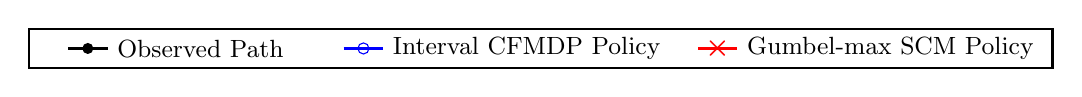
\begin{tikzpicture}[scale=1.0, every node/.style={scale=1.0}]
            \draw[thick, black] (-3, -0.25) rectangle (10, 0.25);
            %
            \draw[black, line width=1pt] (-2.5, 0.0) -- (-2,0.0);
            \fill[black] (-2.25,0.0) circle (2pt); %
            \node[right] at (-2,0.0) {\small Observed Path};
            
            %
            \draw[blue, line width=1pt] (1.0,0.0) -- (1.5,0.0);
            \node[draw=blue, circle, minimum size=4pt, inner sep=0pt] at (1.25,0.0) {}; %
            \node[right] at (1.5,0.0) {\small Interval CFMDP Policy};
            
            %
            \draw[red, line width=1pt] (5.5,0) -- (6,0);
            \node[red] at (5.75,0) {$\boldsymbol{\times}$}; %
            \node[right] at (6,0) {\small Gumbel-max SCM Policy};
        \end{tikzpicture}
    }\\
    %
    \subfigure[\footnotesize Lowest cumulative reward: Interval CFMDP ($312$), Gumbel-max SCM ($312$)]{%
        \resizebox{0.76\columnwidth}{!}{
             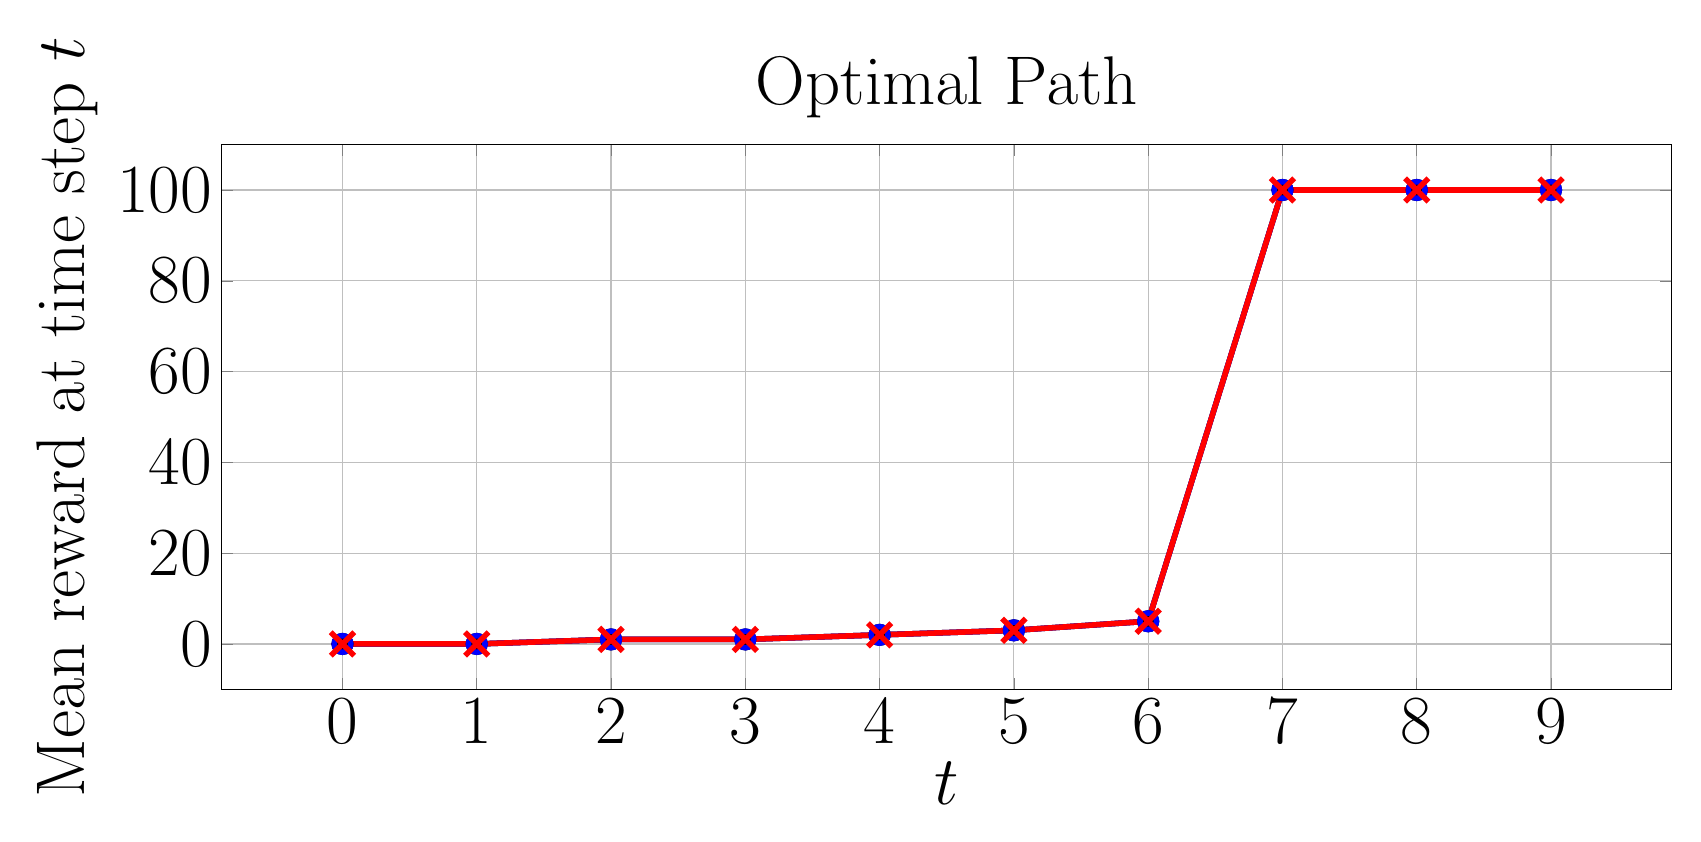
\begin{tikzpicture}
                \begin{axis}[
                    xlabel={$t$},
                    ylabel={Mean reward at time step $t$},
                    title={Optimal Path},
                    grid=both,
                    width=20cm, height=8.5cm,
                    every axis/.style={font=\Huge},
                    %
                ]
                \addplot[
                    color=black, %
                    mark=*, %
                    line width=2pt,
                    mark size=3pt,
                    error bars/.cd,
                    y dir=both, %
                    y explicit, %
                    error bar style={line width=1pt,solid},
                    error mark options={line width=1pt,mark size=4pt,rotate=90}
                ]
                coordinates {
                    (0, 0.0)  +- (0, 0.0)
                    (1, 0.0)  +- (0, 0.0) 
                    (2, 1.0)  +- (0, 0.0) 
                    (3, 1.0)  +- (0, 0.0)
                    (4, 2.0)  +- (0, 0.0)
                    (5, 3.0) +- (0, 0.0)
                    (6, 5.0) +- (0, 0.0)
                    (7, 100.0) +- (0, 0.0)
                    (8, 100.0) +- (0, 0.0)
                    (9, 100.0) +- (0, 0.0)
                };
                %
                \addplot[
                    color=blue, %
                    mark=o, %
                    line width=2pt,
                    mark size=3pt,
                    error bars/.cd,
                    y dir=both, %
                    y explicit, %
                    error bar style={line width=1pt,solid},
                    error mark options={line width=1pt,mark size=4pt,rotate=90}
                ]
                 coordinates {
                    (0, 0.0)  +- (0, 0.0)
                    (1, 0.0)  +- (0, 0.0) 
                    (2, 1.0)  +- (0, 0.0) 
                    (3, 1.0)  +- (0, 0.0)
                    (4, 2.0)  +- (0, 0.0)
                    (5, 3.0) +- (0, 0.0)
                    (6, 5.0) +- (0, 0.0)
                    (7, 100.0) +- (0, 0.0)
                    (8, 100.0) +- (0, 0.0)
                    (9, 100.0) +- (0, 0.0)
                };
                %
                \addplot[
                    color=red, %
                    mark=x, %
                    line width=2pt,
                    mark size=6pt,
                    error bars/.cd,
                    y dir=both, %
                    y explicit, %
                    error bar style={line width=1pt,solid},
                    error mark options={line width=1pt,mark size=4pt,rotate=90}
                ]
                coordinates {
                    (0, 0.0)  +- (0, 0.0)
                    (1, 0.0)  +- (0, 0.0) 
                    (2, 1.0)  +- (0, 0.0) 
                    (3, 1.0)  +- (0, 0.0)
                    (4, 2.0)  +- (0, 0.0)
                    (5, 3.0) +- (0, 0.0)
                    (6, 5.0) +- (0, 0.0)
                    (7, 100.0) +- (0, 0.0)
                    (8, 100.0) +- (0, 0.0)
                    (9, 100.0) +- (0, 0.0)
                };
                \end{axis}
            \end{tikzpicture}
         }
    }
    \hspace{1cm}
    \subfigure[\footnotesize Lowest cumulative reward: Interval CFMDP ($19$), Gumbel-max SCM ($-88$)]{%
         \resizebox{0.76\columnwidth}{!}{
            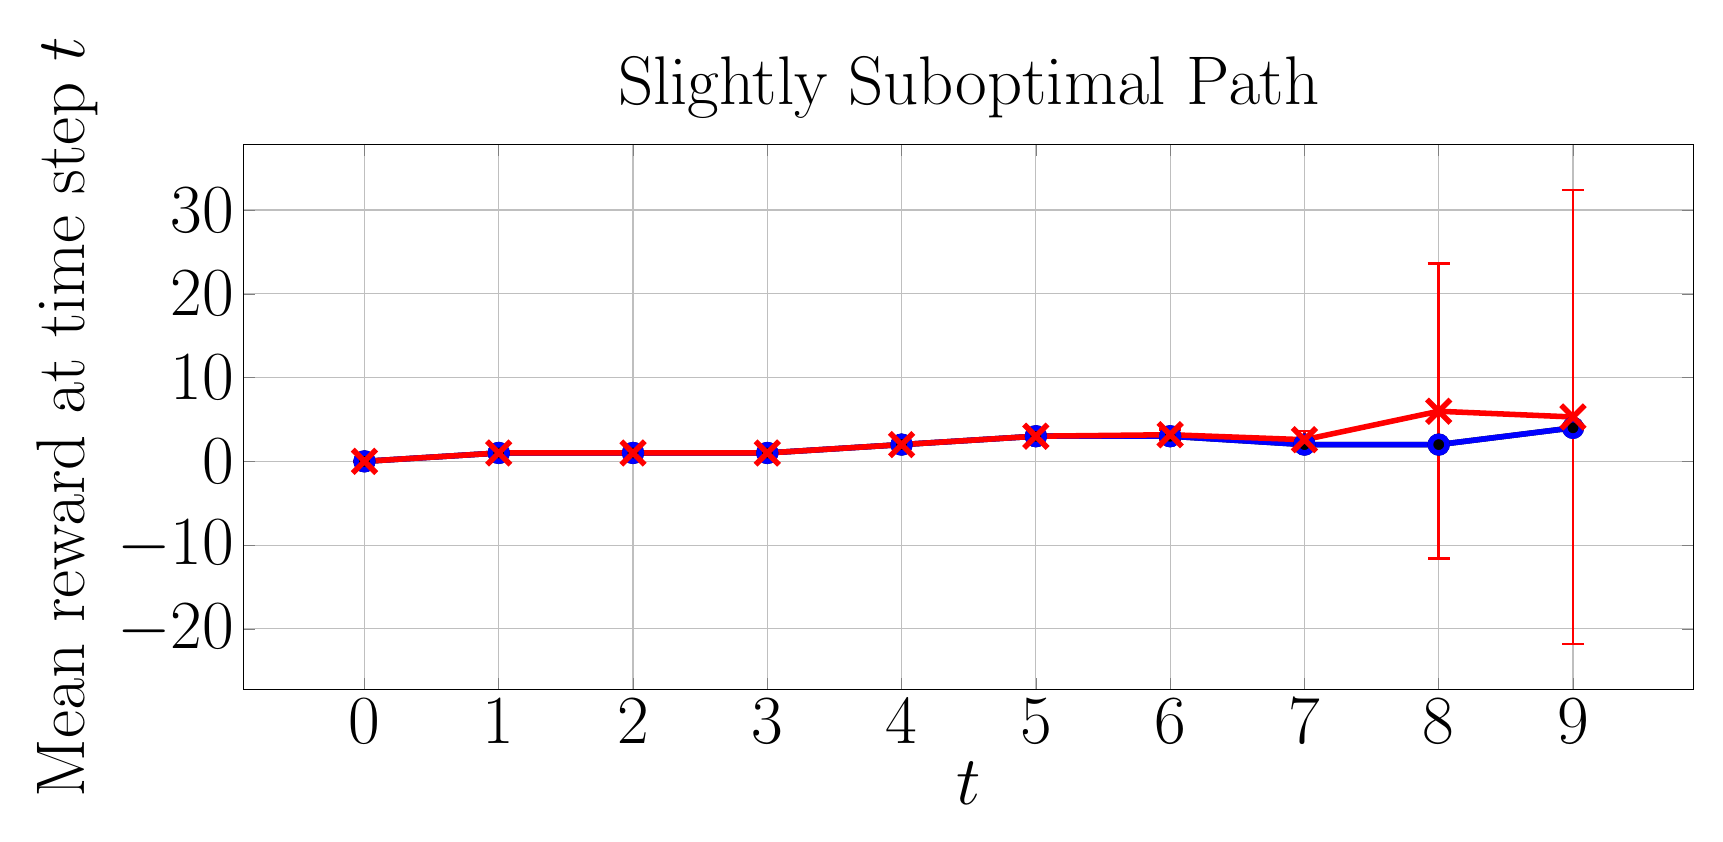
\begin{tikzpicture}
                \begin{axis}[
                    xlabel={$t$},
                    ylabel={Mean reward at time step $t$},
                    title={Slightly Suboptimal Path},
                    grid=both,
                    width=20cm, height=8.5cm,
                    every axis/.style={font=\Huge},
                    %
                ]
                \addplot[
                    color=black, %
                    mark=*, %
                    line width=2pt,
                    mark size=3pt,
                    error bars/.cd,
                    y dir=both, %
                    y explicit, %
                    error bar style={line width=1pt,solid},
                    error mark options={line width=1pt,mark size=4pt,rotate=90}
                ]
              coordinates {
                    (0, 0.0)  +- (0, 0.0)
                    (1, 1.0)  +- (0, 0.0) 
                    (2, 1.0)  +- (0, 0.0) 
                    (3, 1.0)  +- (0, 0.0)
                    (4, 2.0)  +- (0, 0.0)
                    (5, 3.0) +- (0, 0.0)
                    (6, 3.0) +- (0, 0.0)
                    (7, 2.0) +- (0, 0.0)
                    (8, 2.0) +- (0, 0.0)
                    (9, 4.0) +- (0, 0.0)
                };
                %
                \addplot[
                    color=blue, %
                    mark=o, %
                    line width=2pt,
                    mark size=3pt,
                    error bars/.cd,
                    y dir=both, %
                    y explicit, %
                    error bar style={line width=1pt,solid},
                    error mark options={line width=1pt,mark size=4pt,rotate=90}
                ]
              coordinates {
                    (0, 0.0)  +- (0, 0.0)
                    (1, 1.0)  +- (0, 0.0) 
                    (2, 1.0)  +- (0, 0.0) 
                    (3, 1.0)  +- (0, 0.0)
                    (4, 2.0)  +- (0, 0.0)
                    (5, 3.0) +- (0, 0.0)
                    (6, 3.0) +- (0, 0.0)
                    (7, 2.0) +- (0, 0.0)
                    (8, 2.0) +- (0, 0.0)
                    (9, 4.0) +- (0, 0.0)
                };
                %
                \addplot[
                    color=red, %
                    mark=x, %
                    line width=2pt,
                    mark size=6pt,
                    error bars/.cd,
                    y dir=both, %
                    y explicit, %
                    error bar style={line width=1pt,solid},
                    error mark options={line width=1pt,mark size=4pt,rotate=90}
                ]
                coordinates {
                    (0, 0.0)  +- (0, 0.0)
                    (1, 1.0)  +- (0, 0.0) 
                    (2, 1.0)  +- (0, 0.0) 
                    (3, 1.0)  +- (0, 0.0)
                    (4, 2.0)  += (0, 0.0)
                    (5, 3.0)  += (0, 0.0)
                    (6, 3.17847) += (0, 0.62606746) -= (0, 0.62606746)
                    (7, 2.5832885) += (0, 1.04598233) -= (0, 1.04598233)
                    (8, 5.978909) += (0, 17.60137623) -= (0, 17.60137623)
                    (9, 5.297059) += (0, 27.09227512) -= (0, 27.09227512)
                };
                \end{axis}
            \end{tikzpicture}
         }
    }\\[-1.5pt]
    \subfigure[\footnotesize Lowest cumulative reward: Interval CFMDP ($14$), Gumbel-max SCM ($-598$)]{%
         \resizebox{0.76\columnwidth}{!}{
             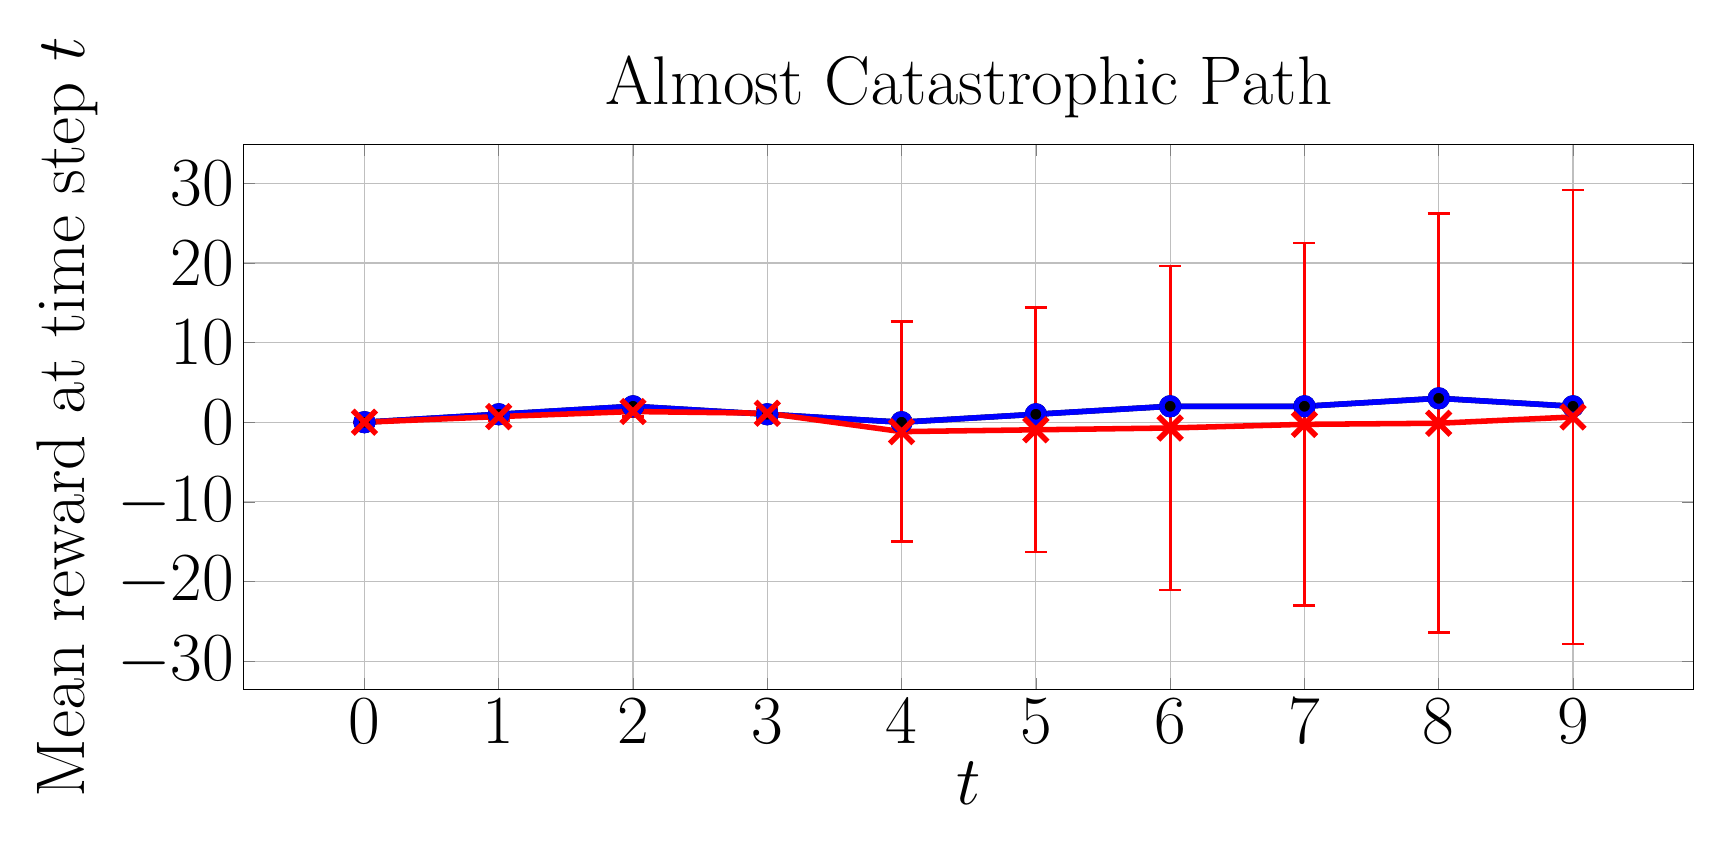
\begin{tikzpicture}
                \begin{axis}[
                    xlabel={$t$},
                    ylabel={Mean reward at time step $t$},
                    title={Almost Catastrophic Path},
                    grid=both,
                    width=20cm, height=8.5cm,
                    every axis/.style={font=\Huge},
                    %
                ]
                \addplot[
                    color=black, %
                    mark=*, %
                    line width=2pt,
                    mark size=3pt,
                    error bars/.cd,
                    y dir=both, %
                    y explicit, %
                    error bar style={line width=1pt,solid},
                    error mark options={line width=1pt,mark size=4pt,rotate=90}
                ]
                coordinates {
                    (0, 0.0)  +- (0, 0.0)
                    (1, 1.0)  +- (0, 0.0) 
                    (2, 2.0)  +- (0, 0.0) 
                    (3, 1.0)  +- (0, 0.0)
                    (4, 0.0)  +- (0, 0.0)
                    (5, 1.0) +- (0, 0.0)
                    (6, 2.0) +- (0, 0.0)
                    (7, 2.0) +- (0, 0.0)
                    (8, 3.0) +- (0, 0.0)
                    (9, 2.0) +- (0, 0.0)
                };
                %
                \addplot[
                    color=blue, %
                    mark=o, %
                    line width=2pt,
                    mark size=3pt,
                    error bars/.cd,
                    y dir=both, %
                    y explicit, %
                    error bar style={line width=1pt,solid},
                    error mark options={line width=1pt,mark size=4pt,rotate=90}
                ]
                coordinates {
                    (0, 0.0)  +- (0, 0.0)
                    (1, 1.0)  +- (0, 0.0) 
                    (2, 2.0)  +- (0, 0.0) 
                    (3, 1.0)  +- (0, 0.0)
                    (4, 0.0)  +- (0, 0.0)
                    (5, 1.0) +- (0, 0.0)
                    (6, 2.0) +- (0, 0.0)
                    (7, 2.0) +- (0, 0.0)
                    (8, 3.0) +- (0, 0.0)
                    (9, 2.0) +- (0, 0.0)
                };
                %
                \addplot[
                    color=red, %
                    mark=x, %
                    line width=2pt,
                    mark size=6pt,
                    error bars/.cd,
                    y dir=both, %
                    y explicit, %
                    error bar style={line width=1pt,solid},
                    error mark options={line width=1pt,mark size=4pt,rotate=90}
                ]
                coordinates {
                    (0, 0.0)  +- (0, 0.0)
                    (1, 0.7065655)  +- (0, 0.4553358) 
                    (2, 1.341673)  +- (0, 0.67091621) 
                    (3, 1.122926)  +- (0, 0.61281824)
                    (4, -1.1821935)  +- (0, 13.82444042)
                    (5, -0.952399)  +- (0, 15.35195457)
                    (6, -0.72672) +- (0, 20.33508414)
                    (7, -0.268983) +- (0, 22.77861454)
                    (8, -0.1310835) +- (0, 26.31013314)
                    (9, 0.65806) +- (0, 28.50670214)
                };
                %
            %
            %
            %
            %
            %
            %
            %
            %
            %
            %
            %
            %
            %
            %
            %
            %
            %
            %
                \end{axis}
            \end{tikzpicture}
         }
    }
    \hspace{1cm}
    \subfigure[\footnotesize Lowest cumulative reward: Interval CFMDP ($-698$), Gumbel-max SCM ($-698$)]{%
         \resizebox{0.76\columnwidth}{!}{
            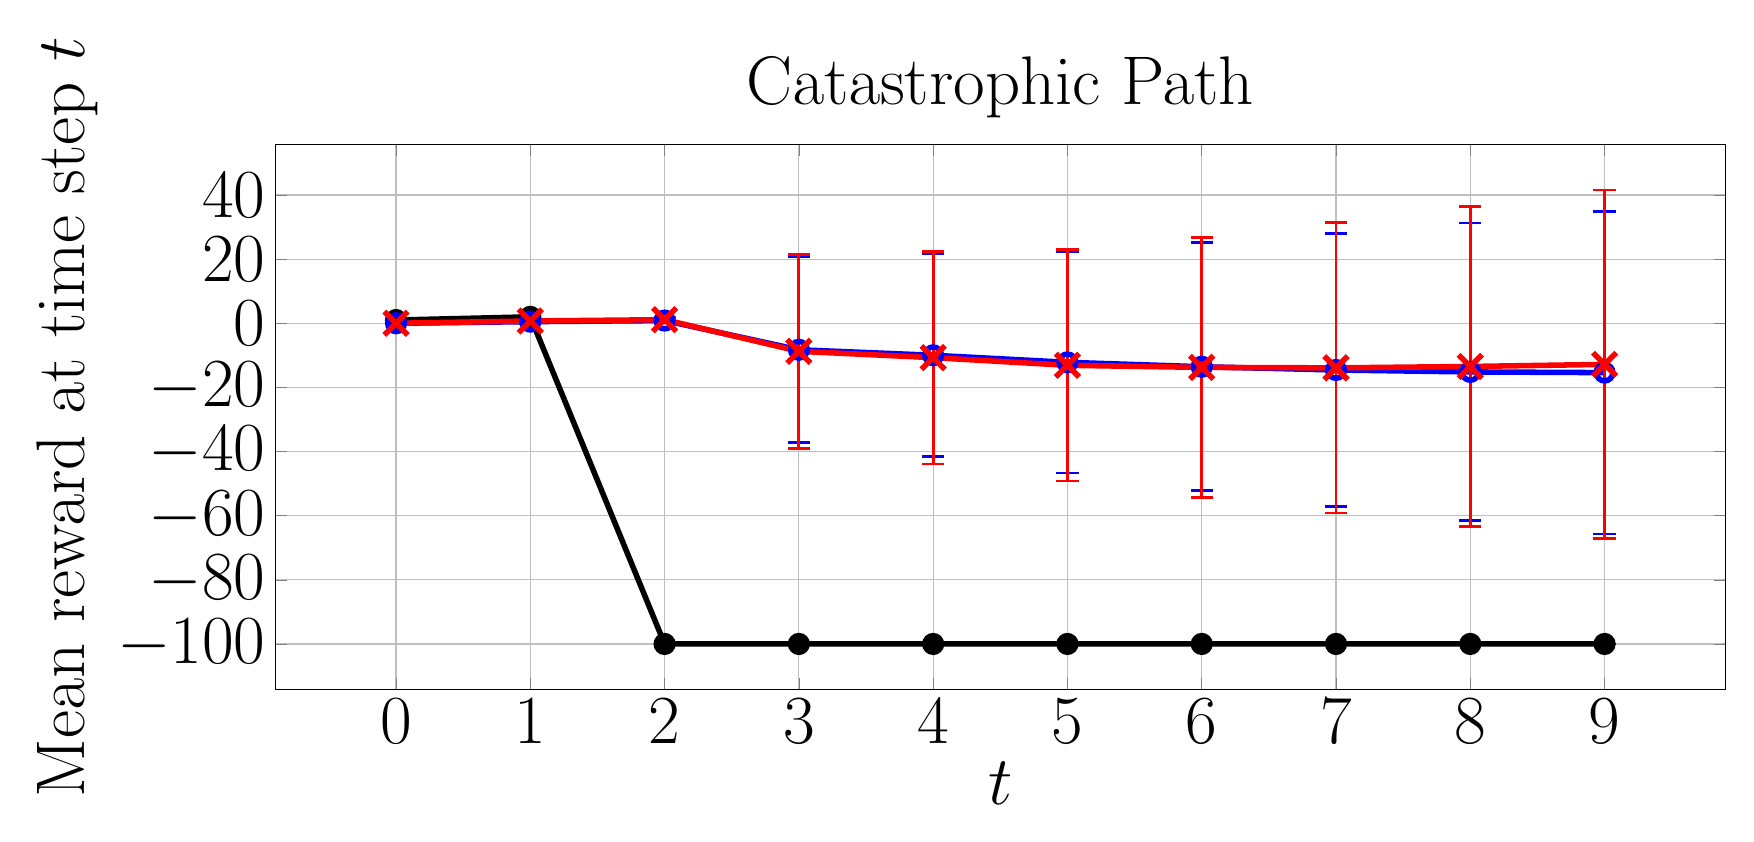
\begin{tikzpicture}
                \begin{axis}[
                    xlabel={$t$},
                    ylabel={Mean reward at time step $t$},
                    title={Catastrophic Path},
                    grid=both,
                    width=20cm, height=8.5cm,
                    every axis/.style={font=\Huge},
                    %
                ]
                \addplot[
                    color=black, %
                    mark=*, %
                    line width=2pt,
                    mark size=3pt,
                    error bars/.cd,
                    y dir=both, %
                    y explicit, %
                    error bar style={line width=1pt,solid},
                    error mark options={line width=1pt,mark size=4pt,rotate=90}
                ]
                coordinates {
                    (0, 1.0)  +- (0, 0.0)
                    (1, 2.0)  +- (0, 0.0) 
                    (2, -100.0)  +- (0, 0.0) 
                    (3, -100.0)  +- (0, 0.0)
                    (4, -100.0)  +- (0, 0.0)
                    (5, -100.0) +- (0, 0.0)
                    (6, -100.0) +- (0, 0.0)
                    (7, -100.0) +- (0, 0.0)
                    (8, -100.0) +- (0, 0.0)
                    (9, -100.0) +- (0, 0.0)
                };
                %
                \addplot[
                    color=blue, %
                    mark=o, %
                    line width=2pt,
                    mark size=3pt,
                    error bars/.cd,
                    y dir=both, %
                    y explicit, %
                    error bar style={line width=1pt,solid},
                    error mark options={line width=1pt,mark size=4pt,rotate=90}
                ]
                coordinates {
                    (0, 0.0)  +- (0, 0.0)
                    (1, 0.504814)  +- (0, 0.49997682) 
                    (2, 0.8439835)  +- (0, 0.76831917) 
                    (3, -8.2709165)  +- (0, 28.93656754)
                    (4, -9.981082)  +- (0, 31.66825363)
                    (5, -12.1776325) +- (0, 34.53463233)
                    (6, -13.556076) +- (0, 38.62845372)
                    (7, -14.574418) +- (0, 42.49603359)
                    (8, -15.1757075) +- (0, 46.41913968)
                    (9, -15.3900395) +- (0, 50.33563368)
                };
                %
                \addplot[
                    color=red, %
                    mark=x, %
                    line width=2pt,
                    mark size=6pt,
                    error bars/.cd,
                    y dir=both, %
                    y explicit, %
                    error bar style={line width=1pt,solid},
                    error mark options={line width=1pt,mark size=4pt,rotate=90}
                ]
                coordinates {
                    (0, 0.0)  +- (0, 0.0)
                    (1, 0.701873)  +- (0, 0.45743556) 
                    (2, 1.1227805)  +- (0, 0.73433129) 
                    (3, -8.7503255)  +- (0, 30.30257976)
                    (4, -10.722092)  +- (0, 33.17618589)
                    (5, -13.10721)  +- (0, 36.0648089)
                    (6, -13.7631645) +- (0, 40.56553451)
                    (7, -13.909043) +- (0, 45.23829402)
                    (8, -13.472517) +- (0, 49.96270296)
                    (9, -12.8278835) +- (0, 54.38618735)
                };
                %
            %
            %
            %
            %
            %
            %
            %
            %
            %
            %
            %
            %
            %
            %
            %
            %
            %
            %
                \end{axis}
            \end{tikzpicture}
         }
    }
    \caption{Average instant reward of CF paths induced by policies on GridWorld $p=0.4$.}
    \label{fig: reward p=0.4}
\end{figure*}

\subsection{Experimental Setup}
To compare policy performance, we measure the average rewards of counterfactual paths induced by our policy and the Gumbel-max policy by uniformly sampling $200$ counterfactual MDPs from the ICFMDP and generating $10,000$ counterfactual paths over each sampled CFMDP. \jl{Since the interval CFMDP depends on the observed path, we select $4$  paths of varying optimality to evaluate how the observed path impacts the performance of both policies: an optimal path, a slightly suboptimal path that could reach the optimal reward with a few changes, a catastrophic path that enters a catastrophic, terminal state with low reward, and an almost catastrophic path that was close to entering a catastrophic state.} When measuring the average probability bound widths and execution time needed to generate the ICFMDPs, we averaged over $20$ randomly generated observed paths
\footnote{Further training details are provided in Appendix \ref{app: training details}, and the code is provided at \href{https://github.com/ddv-lab/robust-cf-inference-in-MDPs}{https://github.com/ddv-lab/robust-cf-inference-in-MDPs}
%
%
.}.

\subsection{GridWorld}
\jl{The GridWorld MDP is a $4 \times 4$ grid where an agent must navigate from the top-left corner to the goal state in the bottom-right corner, avoiding a dangerous terminal state in the centre. At each time step, the agent can move up, down, left, or right, but there is a small probability (controlled by hyper-parameter $p$) of moving in an unintended direction. As the agent nears the goal, the reward for each state increases, culminating in a reward of $+100$ for reaching the goal. Entering the dangerous state results in a penalty of $-100$. We use two versions of GridWorld: a less stochastic version with $p=0.9$ (i.e., $90$\% chance of moving in the chosen direction) and a more stochastic version with $p=0.4$.}

\paragraph{GridWorld ($p=0.9$)}
When $p=0.9$, the counterfactual probability bounds are typically narrow (see Table \ref{tab:nonzero_probs} for average measurements). Consequently, as shown in Figure \ref{fig: reward p=0.9}, both policies are nearly identical and perform similarly well across the optimal, slightly suboptimal, and catastrophic paths.
%
However, for the almost catastrophic path, the interval CFMDP path is more conservative and follows the observed path more closely (as this is where the probability bounds are narrowest), which typically requires one additional step to reach the goal state than the Gumbel-max SCM policy.
%

\paragraph{GridWorld ($p=0.4$)}
\jl{When $p=0.4$, the GridWorld environment becomes more uncertain, increasing the risk of entering the dangerous state even if correct actions are chosen. Thus, as shown in Figure \ref{fig: reward p=0.4}, the interval CFMDP policy adopts a more conservative approach, avoiding deviation from the observed policy if it cannot guarantee higher counterfactual rewards (see the slightly suboptimal and almost catastrophic paths), whereas the Gumbel-max SCM is inconsistent: it can yield higher rewards, but also much lower rewards, reflected in the wide error bars.} For the catastrophic path, both policies must deviate from the observed path to achieve a higher reward and, in this case, perform similarly.
%
%
%
%
\subsection{Sepsis}
The Sepsis MDP \citep{oberst2019counterfactual} simulates trajectories of Sepsis patients. Each state consists of four vital signs (heart rate, blood pressure, oxygen concentration, and glucose levels), categorised as low, normal, or high.
and three treatments that can be toggled on/off at each time step (8 actions in total). Unlike \citet{oberst2019counterfactual}, we scale rewards based on the number of out-of-range vital signs, between $-1000$ (patient dies) and $1000$ (patient discharged). \jl{Like the GridWorld $p=0.4$ experiment, the Sepsis MDP is highly uncertain, as many states are equally likely to lead to optimal and poor outcomes. Thus, as shown in Figure \ref{fig: reward sepsis}, both policies follow the observed optimal and almost catastrophic paths to guarantee rewards are no worse than the observation.} However, improving the catastrophic path requires deviating from the observation. Here, the Gumbel-max SCM policy, on average, performs better than the interval CFMDP policy. But, since both policies have lower bounds clipped at $-1000$, neither policy reliably improves over the observation. In contrast, for the slightly suboptimal path, the interval CFMDP policy performs significantly better, shown by its higher lower bounds. 
Moreover, in these two cases, the worst-case counterfactual path generated by the interval CFMDP policy is better than that of the Gumbel-max SCM policy,
indicating its greater robustness.
%
\begin{figure*}
    \centering
     \resizebox{0.6\textwidth}{!}{
        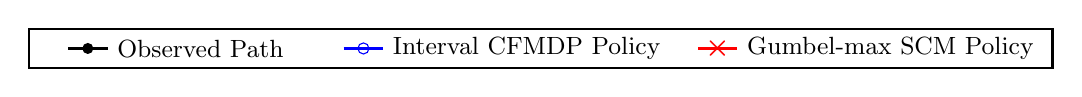
\begin{tikzpicture}[scale=1.0, every node/.style={scale=1.0}]
            \draw[thick, black] (-3, -0.25) rectangle (10, 0.25);
            %
            \draw[black, line width=1pt] (-2.5, 0.0) -- (-2,0.0);
            \fill[black] (-2.25,0.0) circle (2pt); %
            \node[right] at (-2,0.0) {\small Observed Path};
            
            %
            \draw[blue, line width=1pt] (1.0,0.0) -- (1.5,0.0);
            \node[draw=blue, circle, minimum size=4pt, inner sep=0pt] at (1.25,0.0) {}; %
            \node[right] at (1.5,0.0) {\small Interval CFMDP Policy};
            
            %
            \draw[red, line width=1pt] (5.5,0) -- (6,0);
            \node[red] at (5.75,0) {$\boldsymbol{\times}$}; %
            \node[right] at (6,0) {\small Gumbel-max SCM Policy};
        \end{tikzpicture}
    }\\
    \subfigure[\footnotesize Lowest cumulative reward: Interval CFMDP ($8000$), Gumbel-max SCM ($8000$)]{%
         \resizebox{0.76\columnwidth}{!}{
             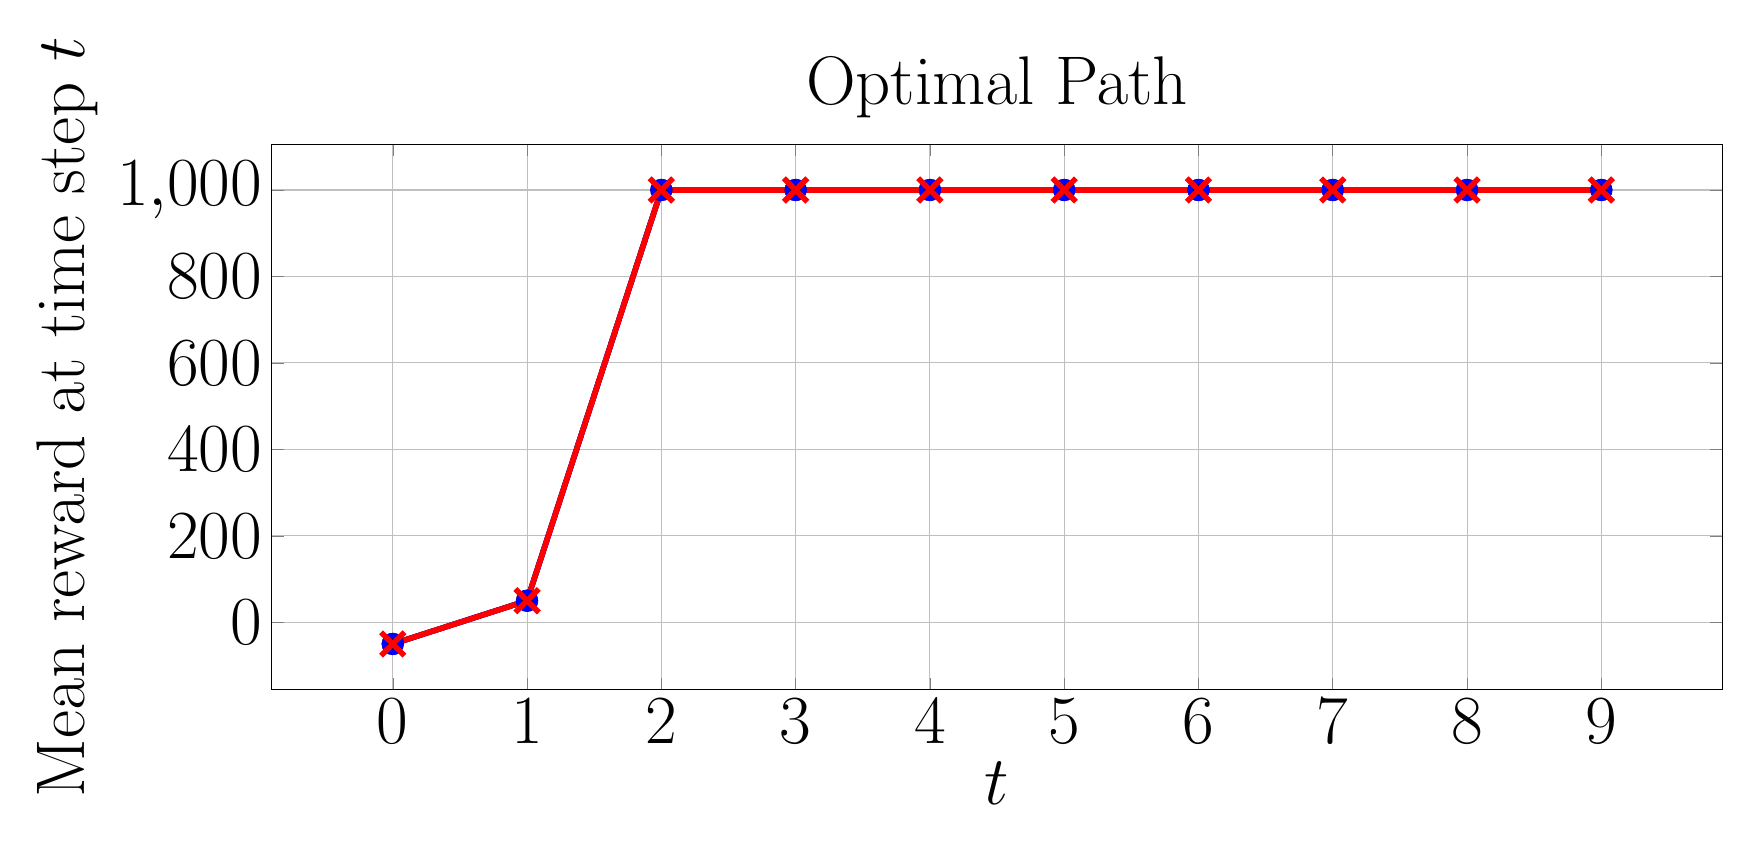
\begin{tikzpicture}
                \begin{axis}[
                    xlabel={$t$},
                    ylabel={Mean reward at time step $t$},
                    title={Optimal Path},
                    grid=both,
                    width=20cm, height=8.5cm,
                    every axis/.style={font=\Huge},
                    %
                ]
                \addplot[
                    color=black, %
                    mark=*, %
                    line width=2pt,
                    mark size=3pt,
                ]
                coordinates {
                    (0, -50.0)
                    (1, 50.0)
                    (2, 1000.0)
                    (3, 1000.0)
                    (4, 1000.0)
                    (5, 1000.0)
                    (6, 1000.0)
                    (7, 1000.0)
                    (8, 1000.0)
                    (9, 1000.0)
                };
                %
                \addplot[
                    color=blue, %
                    mark=o, %
                    line width=2pt,
                    mark size=3pt,
                    error bars/.cd,
                    y dir=both, %
                    y explicit, %
                    error bar style={line width=1pt,solid},
                    error mark options={line width=1pt,mark size=4pt,rotate=90}
                ]
                coordinates {
                    (0, -50.0)  +- (0, 0.0)
                    (1, 50.0)  +- (0, 0.0) 
                    (2, 1000.0)  +- (0, 0.0) 
                    (3, 1000.0)  +- (0, 0.0)
                    (4, 1000.0)  +- (0, 0.0)
                    (5, 1000.0) +- (0, 0.0)
                    (6, 1000.0) +- (0, 0.0)
                    (7, 1000.0) +- (0, 0.0)
                    (8, 1000.0) +- (0, 0.0)
                    (9, 1000.0) +- (0, 0.0)
                };
                %
                \addplot[
                    color=red, %
                    mark=x, %
                    line width=2pt,
                    mark size=6pt,
                    error bars/.cd,
                    y dir=both, %
                    y explicit, %
                    error bar style={line width=1pt,solid},
                    error mark options={line width=1pt,mark size=4pt,rotate=90}
                ]
                coordinates {
                    (0, -50.0)  +- (0, 0.0)
                    (1, 50.0)  +- (0, 0.0) 
                    (2, 1000.0)  +- (0, 0.0) 
                    (3, 1000.0)  +- (0, 0.0)
                    (4, 1000.0)  +- (0, 0.0)
                    (5, 1000.0) +- (0, 0.0)
                    (6, 1000.0) +- (0, 0.0)
                    (7, 1000.0) +- (0, 0.0)
                    (8, 1000.0) +- (0, 0.0)
                    (9, 1000.0) +- (0, 0.0)
                };
                %
                \end{axis}
            \end{tikzpicture}
         }
    }
    \hspace{1cm}
    \subfigure[\footnotesize Lowest cumulative reward: Interval CFMDP ($-5980$), Gumbel-max SCM ($-8000$)]{%
         \resizebox{0.76\columnwidth}{!}{
            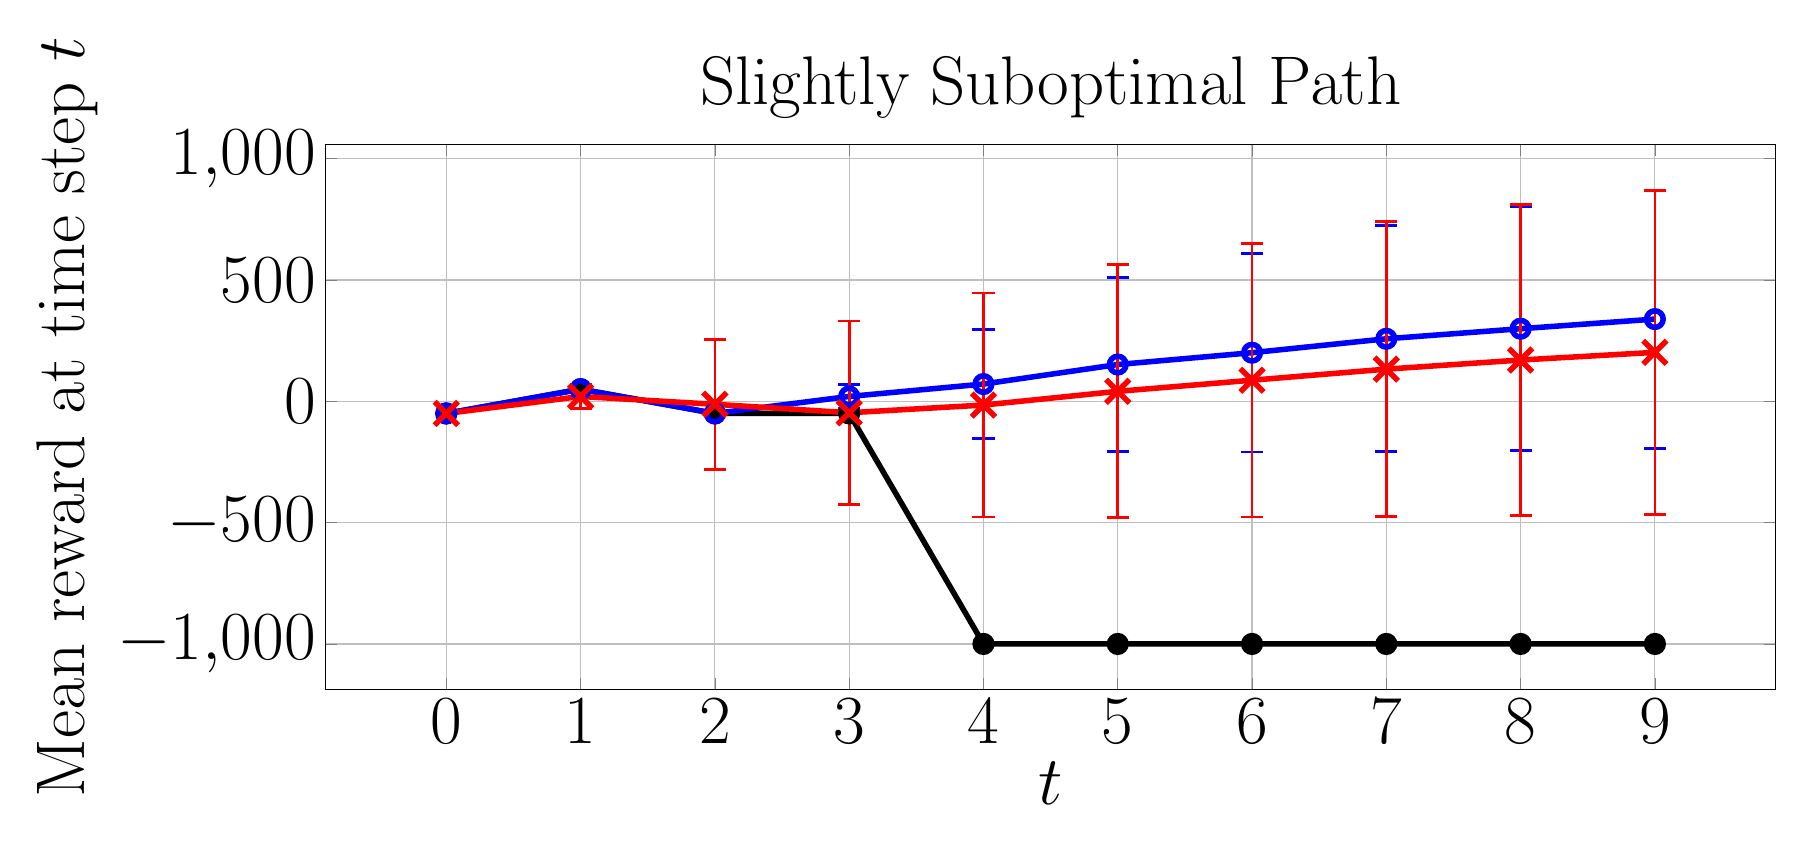
\begin{tikzpicture}
                \begin{axis}[
                    xlabel={$t$},
                    ylabel={Mean reward at time step $t$},
                    title={Slightly Suboptimal Path},
                    grid=both,
                    width=20cm, height=8.5cm,
                    every axis/.style={font=\Huge},
                    %
                ]
               \addplot[
                    color=black, %
                    mark=*, %
                    line width=2pt,
                    mark size=3pt,
                ]
                coordinates {
                    (0, -50.0)
                    (1, 50.0)
                    (2, -50.0)
                    (3, -50.0)
                    (4, -1000.0)
                    (5, -1000.0)
                    (6, -1000.0)
                    (7, -1000.0)
                    (8, -1000.0)
                    (9, -1000.0)
                };
                %
                \addplot[
                    color=blue, %
                    mark=o, %
                    line width=2pt,
                    mark size=3pt,
                    error bars/.cd,
                    y dir=both, %
                    y explicit, %
                    error bar style={line width=1pt,solid},
                    error mark options={line width=1pt,mark size=4pt,rotate=90}
                ]
                coordinates {
                    (0, -50.0)  +- (0, 0.0)
                    (1, 50.0)  +- (0, 0.0) 
                    (2, -50.0)  +- (0, 0.0) 
                    (3, 20.0631)  +- (0, 49.97539413)
                    (4, 71.206585)  +- (0, 226.02033693)
                    (5, 151.60797) +- (0, 359.23292559)
                    (6, 200.40593) +- (0, 408.86185176)
                    (7, 257.77948) +- (0, 466.10372804)
                    (8, 299.237465) +- (0, 501.82579506)
                    (9, 338.9129) +- (0, 532.06124996)
                };
                %
                \addplot[
                    color=red, %
                    mark=x, %
                    line width=2pt,
                    mark size=6pt,
                    error bars/.cd,
                    y dir=both, %
                    y explicit, %
                    error bar style={line width=1pt,solid},
                    error mark options={line width=1pt,mark size=4pt,rotate=90}
                ]
                coordinates {
                    (0, -50.0)  +- (0, 0.0)
                    (1, 20.00736)  +- (0, 49.99786741) 
                    (2, -12.282865)  +- (0, 267.598755) 
                    (3, -47.125995)  +- (0, 378.41755832)
                    (4, -15.381965)  +- (0, 461.77616558)
                    (5, 41.15459) +- (0, 521.53189262)
                    (6, 87.01595) +- (0, 564.22243126 )
                    (7, 132.62376) +- (0, 607.31338037)
                    (8, 170.168145) +- (0, 641.48013693)
                    (9, 201.813135) +- (0, 667.29441777)
                };
                %
                %
                %
                %
                %
                %
                %
                %
                %
                %
                %
                %
                %
                %
                %
                %
                %
                %
                %
                \end{axis}
            \end{tikzpicture}
         }
    }\\[-1.5pt]
    \subfigure[\footnotesize Lowest cumulative reward: Interval CFMDP ($100$), Gumbel-max SCM ($100$)]{%
         \resizebox{0.76\columnwidth}{!}{
             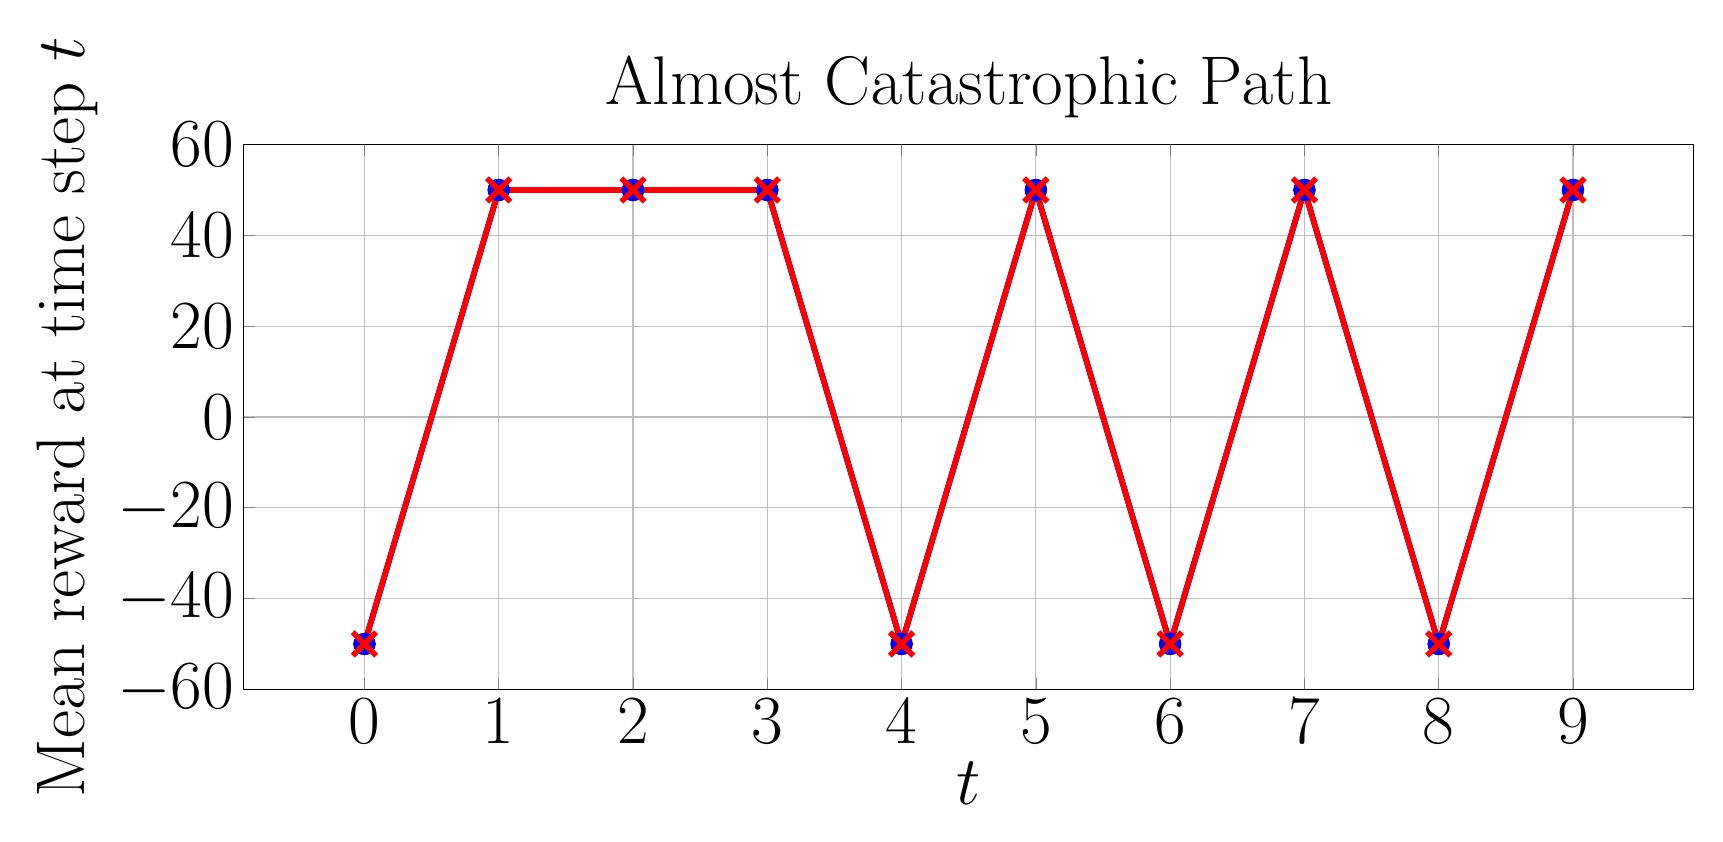
\begin{tikzpicture}
                \begin{axis}[
                    xlabel={$t$},
                    ylabel={Mean reward at time step $t$},
                    title={Almost Catastrophic Path},
                    grid=both,
                    every axis/.style={font=\Huge},
                    width=20cm, height=8.5cm,
                    %
                ]
               \addplot[
                    color=black, %
                    mark=*, %
                    line width=2pt,
                    mark size=3pt,
                ]
                coordinates {
                    (0, -50.0)
                    (1, 50.0)
                    (2, 50.0)
                    (3, 50.0)
                    (4, -50.0)
                    (5, 50.0)
                    (6, -50.0)
                    (7, 50.0)
                    (8, -50.0)
                    (9, 50.0)
                };
                %
                %
                \addplot[
                    color=blue, %
                    mark=o, %
                    line width=2pt,
                    mark size=3pt,
                    error bars/.cd,
                    y dir=both, %
                    y explicit, %
                    error bar style={line width=1pt,solid},
                    error mark options={line width=1pt,mark size=4pt,rotate=90}
                ]
                coordinates {
                    (0, -50.0)  +- (0, 0.0)
                    (1, 50.0)  +- (0, 0.0) 
                    (2, 50.0)  +- (0, 0.0) 
                    (3, 50.0)  +- (0, 0.0)
                    (4, -50.0)  +- (0, 0.0)
                    (5, 50.0) +- (0, 0.0)
                    (6, -50.0) +- (0, 0.0)
                    (7, 50.0) +- (0, 0.0)
                    (8, -50.0) +- (0, 0.0)
                    (9, 50.0) +- (0, 0.0)
                };
                %
                \addplot[
                    color=red, %
                    mark=x, %
                    line width=2pt,
                    mark size=6pt,
                    error bars/.cd,
                    y dir=both, %
                    y explicit, %
                    error bar style={line width=1pt,solid},
                    error mark options={line width=1pt,mark size=4pt,rotate=90}
                ]
                coordinates {
                    (0, -50.0)  +- (0, 0.0)
                    (1, 50.0)  +- (0, 0.0) 
                    (2, 50.0)  +- (0, 0.0) 
                    (3, 50.0)  +- (0, 0.0)
                    (4, -50.0)  +- (0, 0.0)
                    (5, 50.0) +- (0, 0.0)
                    (6, -50.0) +- (0, 0.0)
                    (7, 50.0) +- (0, 0.0)
                    (8, -50.0) +- (0, 0.0)
                    (9, 50.0) +- (0, 0.0)
                };
                %
                %
                %
                %
                %
                %
                %
                %
                %
                %
                %
                %
                %
                %
                %
                %
                %
                %
                %
                \end{axis}
            \end{tikzpicture}
         }
    }
    \hspace{1cm}
    \subfigure[\footnotesize Lowest cumulative reward: Interval CFMDP ($-7150$), Gumbel-max SCM ($-9050$)]{%
         \resizebox{0.76\columnwidth}{!}{
            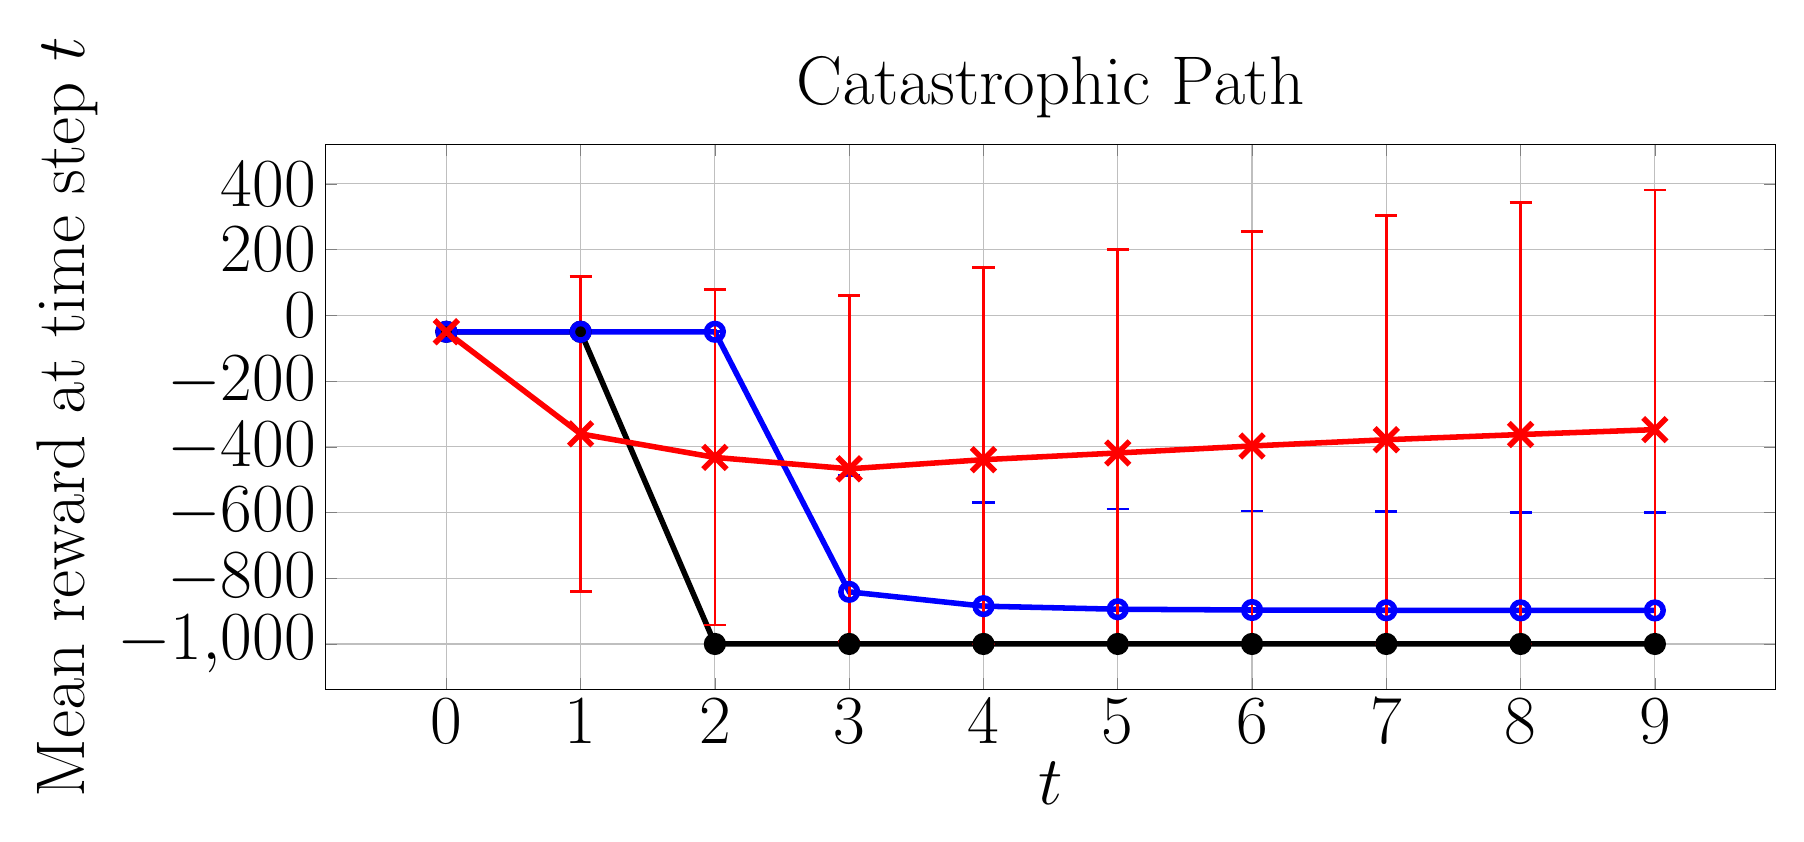
\begin{tikzpicture}
                \begin{axis}[
                    xlabel={$t$},
                    ylabel={Mean reward at time step $t$},
                    title={Catastrophic Path},
                    grid=both,
                    width=20cm, height=8.5cm,
                    every axis/.style={font=\Huge},
                    %
                ]
               \addplot[
                    color=black, %
                    mark=*, %
                    line width=2pt,
                    mark size=3pt,
                ]
                coordinates {
                    (0, -50.0)
                    (1, -50.0)
                    (2, -1000.0)
                    (3, -1000.0)
                    (4, -1000.0)
                    (5, -1000.0)
                    (6, -1000.0)
                    (7, -1000.0)
                    (8, -1000.0)
                    (9, -1000.0)
                };
                %
                %
                \addplot[
                    color=blue, %
                    mark=o, %
                    line width=2pt,
                    mark size=3pt,
                    error bars/.cd,
                    y dir=both, %
                    y explicit, %
                    error bar style={line width=1pt,solid},
                    error mark options={line width=1pt,mark size=4pt,rotate=90}
                ]
                coordinates {
                    (0, -50.0)  +- (0, 0.0)
                    (1, -50.0)  +- (0, 0.0) 
                    (2, -50.0)  +- (0, 0.0) 
                    (3, -841.440725)  += (0, 354.24605512) -= (0, 158.559275)
                    (4, -884.98225)  += (0, 315.37519669) -= (0, 115.01775)
                    (5, -894.330425) += (0, 304.88572805) -= (0, 105.669575)
                    (6, -896.696175) += (0, 301.19954514) -= (0, 103.303825)
                    (7, -897.4635) += (0, 299.61791279) -= (0, 102.5365)
                    (8, -897.77595) += (0, 298.80392585) -= (0, 102.22405)
                    (9, -897.942975) += (0, 298.32920557) -= (0, 102.057025)
                };
                %
                \addplot[
                    color=red, %
                    mark=x, %
                    line width=2pt,
                    mark size=6pt,
                    error bars/.cd,
                    y dir=both, %
                    y explicit, %
                    error bar style={line width=1pt,solid},
                    error mark options={line width=1pt,mark size=4pt,rotate=90}
                ]
            coordinates {
                    (0, -50.0)  +- (0, 0.0)
                    (1, -360.675265)  +- (0, 479.39812699) 
                    (2, -432.27629)  +- (0, 510.38620897) 
                    (3, -467.029545)  += (0, 526.36009628) -= (0, 526.36009628)
                    (4, -439.17429)  += (0, 583.96638919) -= (0, 560.82571)
                    (5, -418.82704) += (0, 618.43027478) -= (0, 581.17296)
                    (6, -397.464895) += (0, 652.67322574) -= (0, 602.535105)
                    (7, -378.49052) += (0, 682.85407033) -= (0, 621.50948)
                    (8, -362.654195) += (0, 707.01412023) -= (0, 637.345805)
                    (9, -347.737935) += (0, 729.29076479) -= (0, 652.262065)
                };
                %
                %
                %
                %
                %
                %
                %
                %
                %
                %
                %
                %
                %
                %
                %
                %
                %
                %
                %
                \end{axis}
            \end{tikzpicture}
         }
    }
    \caption{Average instant reward of CF paths induced by policies on Sepsis.}
    \label{fig: reward sepsis}
\end{figure*}

%
%
%
\subsection{Interval CFMDP Bounds}
%
%
Table \ref{tab:nonzero_probs} presents the mean counterfactual probability bound widths (excluding transitions where the upper bound is $0$) for each MDP, averaged over 20 observed paths. We compare the bounds under counterfactual stability (CS) and monotonicity (M) assumptions, CS alone, and no assumptions. This shows that the assumptions marginally reduce the bound widths, indicating the assumptions tighten the bounds without excluding too many causal models, as intended.
\renewcommand{\arraystretch}{1}

\begin{table}
\centering
\caption{Mean width of counterfactual probability bounds}
\resizebox{0.8\columnwidth}{!}{%
\begin{tabular}{|c|c|c|c|}
\hline
\multirow{2}{*}{\textbf{Environment}} & \multicolumn{3}{c|}{\textbf{Assumptions}} \\ \cline{2-4}
 & \textbf{CS + M} & \textbf{CS} & \textbf{None\tablefootnote{\jl{Equivalent to \citet{li2024probabilities}'s bounds (see Section \ref{sec: equivalence with Li}).}}} \\ \hline
\textbf{GridWorld} ($p=0.9$) & 0.0817 & 0.0977 & 0.100 \\ \hline
\textbf{GridWorld} ($p=0.4$) & 0.552  & 0.638  & 0.646 \\ \hline
\textbf{Sepsis} & 0.138 & 0.140 & 0.140 \\ \hline
\end{tabular}
}
\label{tab:nonzero_probs}
\end{table}


\subsection{Execution Times}
Table \ref{tab: times} compares the average time needed to generate the interval CFMDP vs.\ the Gumbel-max SCM CFMDP for 20 observations.
The GridWorld algorithms were run single-threaded, while the Sepsis experiments were run in parallel.
Generating the interval CFMDP is significantly faster as it uses exact analytical bounds, whereas the Gumbel-max CFMDP requires sampling from the Gumbel distribution to estimate counterfactual transition probabilities. \jl{Since constructing the counterfactual MDP models is the main bottleneck in both approaches, ours is more efficient overall and suitable for larger MDPs.}
\begin{table}
\centering
\caption{Mean execution time to generate CFMDPs}
\resizebox{0.99\columnwidth}{!}{%
\begin{tabular}{|c|c|c|}
\hline
\multirow{2}{*}{\textbf{Environment}} & \multicolumn{2}{c|}{\textbf{Mean Execution Time (s)}} \\ \cline{2-3} 
                                      & \textbf{Interval CFMDP} & \textbf{Gumbel-max CFMDP} \\ \hline
\textbf{GridWorld ($p=0.9$) }                  & 0.261                   & 56.1                      \\ \hline
\textbf{GridWorld ($p=0.4$)  }                 & 0.336                   & 54.5                      \\ \hline
\textbf{Sepsis}                                 & 688                     & 2940                      \\ \hline
\end{tabular}%
}
\label{tab: times}
\end{table}

\section{Limitation}
The use of 3D-printed PLA for structural components improves improving ease of assembly and reduces weight and cost, yet it causes deformation under heavy load, which can diminish end-effector precision. Using metal, such as aluminum, would remedy this problem. Additionally, \robot relies on integrated joint relative encoders, requiring manual initialization in a fixed joint configuration each time the system is powered on. Using absolute joint encoders could significantly improve accuracy and ease of use, although it would increase the overall cost. 

%Reliance on commercially available actuators simplifies integration but imposes constraints on control frequency and customization, further limiting the potential for tailored performance improvements.

% The 6 DoF configuration provides sufficient mobility for most tasks; however, certain bimanual operations could benefit from an additional degree of freedom to handle complex joint constraints more effectively. Furthermore, the limited torque density of commercially available proprioceptive actuators restricts the payload and torque output, making the system less suitability for handling heavier loads or high-torque applications. 

The 6 DoF configuration of the arm provides sufficient mobility for single-arm manipulation tasks, yet it shows a limitation in certain bimanual manipulation problems. Specifically, when \robot holds onto a rigid object with both hands, each arm loses 1 DoF because the hands are fixed to the object during grasping. This leads to an underactuated kinematic chain which has a limited mobility in 3D space. We can achieve more mobility by letting the object slip inside the grippers, yet this renders the grasp less robust and simulation difficult. Therefore, we anticipate that designing a lightweight 3 DoF wrist in place of the current 2 DoF wrist allows a more diverse repertoire of manipulation in bimanual tasks.

Finally, the limited torque density of commercially available proprioceptive actuators restricts the performance. Currently, all of our actuators feature a 1:10 gear ratio, so \robot can handle up to 2.5 kg of payload. To handle a heavier object and manipulate it with higher torque, we expect the actuator to have 1:20$\sim$30 gear ratio, but it is difficult to find an off-the-shelf product that meets our requirements. Customizing the actuator to increase the torque density while minimizing the weight will enable \robot to move faster and handle more diverse objects.

%These constraints highlight opportunities for improvement in future iterations, including alternative materials for enhanced rigidity, custom actuator designs for higher control precision and torque density, the adoption of absolute joint encoders, and optimized configurations to balance dexterity and weight.



\balance
\bibliographystyle{abbrvnat}
\bibliography{main.bib}

\end{document}
